% This template originates from the Cambridge University thesis 
% which is created by Prof Harish Bhanderi.  
% This is template follows the GNU license for Education and training
% purposes. (http://www-h.eng.cam.ac.uk/help/tpl/textprocessing/ThesisStyle/) 
% 
%
% I modified for uses in University of Information Technology 
% Vietnam National University. 

\documentclass[oneside,12pt]{Classes/uitBA}


 \ifpdf
     \pdfinfo { /Title  (Thesis title)
                /Creator (TeX)
                /Producer (pdfTeX)
                /Author (Tran Huynh Minh Tan)
                /CreationDate (D:20130105000000)  %format D:YYYYMMDDhhmmss
                /ModDate (D:20030815213532)
                /Subject (Thesis title)
                /Keywords (PhD, Thesis)}
     \pdfcatalog { /PageMode (/UseOutlines)
                   /OpenAction (fitbh)  }
 \fi
     
  \university{{ĐẠI HỌC QUỐC GIA THÀNH PHỐ HỒ CHÍ MINH\\
               ĐẠI HỌC CÔNG NGHỆ THÔNG TIN}}
  \collegeordept{{KHOA MẠNG MÁY TÍNH \& TRUYỀN THÔNG}}  
  \degree{KỸ SƯ CÔNG NGHỆ THÔNG TIN}   
  \title{NGHIÊN CỨU HỆ THỐNG MOODLE KẾT HỢP CÔNG NGHỆ HTML5 ỨNG DỤNG TRONG VIỆC LUYỆN NGHE MÔN TIẾNG ANH TRÊN MÁY TÍNH BẢNG} 
  \crest{
\includegraphics[scale=.20]{UITLogo}} 
  \supervisor{{TS. NGUYỄN ANH TUẤN }}
  \author{{	
  HỒ NHẬT QUANG - 09520223
  \\TRẦN HUỲNH MINH TÂN - 09520266
           }}   
  \degreedate{Tháng 2 Năm 2014} 
\hbadness=10000
\hfuzz=50pt
\usepackage{StyleFiles/watermark}
\usepackage{url}
\usepackage{listings}

\onehalfspacing

\begin{document}
\maketitle
\setcounter{secnumdepth}{3}
\setcounter{tocdepth}{3}

\frontmatter % book mode only
\pagenumbering{roman}
% 
\begin{dedication}  

Xin dành tặng quyển luận văn này cho ... 

\end{dedication}

 
 
 
\begin{acknowledgements}      

	Trước tiên chúng em xin gửi lời cảm ơn chân thành và sâu sắc đến các thầy cô giảng viên trường Đại Học Cộng Nghệ Thông Tin nói chung và các thầy cô trong khoa Mạng máy tính Và Truyền thông nói riêng đã tận tình giảng dạy truyền đạt cho chúng em những kiến thức, kinh nghiệm quý báu trong suốt thời gian qua.

	Đặc biệt chúng em xin gửi lời cảm ơn đến thầy Nguyễn Anh Tuấn vì đã tận tình giúp đỡ, trực tiếp chỉ bảo và hướng dẫn chúng em trong suốt quá trình làm khóa luận. Trong thời gian làm việc với thầy, chúng em đã không những tiếp thu thêm nhiều kiến thức bổ ích mà còn học tập được tinh thần làm việc, thái độ nghiên cứu khoa học nghiêm túc, hiệu quả. Đây là những điều rất cần thiết cho chúng em trong quá trình học tập và công tác sau này.

	Chúng em xin được cảm ơn những người bạn đã gắn bó, chia sẻ rất nhiều kinh nghiệm và những kiến thức, nhất là trong thời gian thực hiện khóa luận, giúp đề tài của nhóm chúng em có thể hoàn thành một cách thành công tốt đẹp nhất.

	Sau cùng chúng con xin gửi lời cảm ơn chân thành đến gia đình cùng những người thân đã giúp cho chúng con có được chỗ dựa tinh thần và tạo điều kiện học tập, nghiên cứu tốt nhất để chúng con hoàn thành khóa luận này.

\end{acknowledgements}
  




\tableofcontents
\listoffigures
% \printnomenclature  
 %\addcontentsline{toc}{chapter}{Nomenclature}
\begin{abstracts}         

Trong bối cảnh thời kỳ mở cửa, đất nước đang trên đà phát triển và hội nhập, ngày càng nhiều các doanh nghiệp nước ngoài đầu tư sang thị trường Việt Nam, mang lại rất nhiều cơ hội việc làm cho các lao động trẻ. Vì vậy, nếu không có một trình độ ngoại ngữ nhất định, người Việt trẻ không thể giành lấy cơ hội ngàn vàng này. Theo những khảo sát thực tế cho thấy, giữa hai người có năng lực chuyên môn ngang nhau, nhà tuyển dụng chắc chắn sẽ lựa chọn người có thêm khả năng ngoại ngữ, nhất là vốn tiếng Anh giao tiếp.

Với mục tiêu hỗ trợ các bạn học sinh – sinh viên có cơ hội phát triển kỹ năng học tiếng Anh nhằm nâng cao khả năng giao tiếp với người nước ngoài, đặc biệt là kỹ năng nghe hiểu, nhóm chúng em quyết định xây dựng “Ứng dụng luyện nghe tiếng Anh” trên thiết bị di động khá phổ biến ngày nay, đó là chiếc máy tính bảng.

\end{abstracts}


\mainmatter  
% \pagebreak[4]
% \hspace*{1cm}
% \pagebreak[4]
% \hspace*{1cm}
% \pagebreak[4]

\chapter{Giới Thiệu}
\ifpdf
    \graphicspath{{Chapter1/Chapter1Figs/PNG/}{Chapter1/Chapter1Figs/PDF/}{Chapter1/Chapter1Figs/}}
\else
    \graphicspath{{Chapter1/Chapter1Figs/EPS/}{Chapter1/Chapter1Figs/}}
\fi

\section{Tên đề tài}

\textbf{	NGHIÊN CỨU HỆ THỐNG MOODLE KẾT HỢP CÔNG NGHỆ HTML5 ỨNG DỤNG TRONG VIỆC LUYỆN NGHE MÔN TIẾNG ANH TRÊN MÁY TÍNH BẢNG.}

\section{Đặt vấn đề}

So với cách học tiếng Anh truyền thống như học gia sư, các trung tâm uy tín, và thường gặp nhất là tự học qua sách báo, giáo trình bán sẵn thì việc học tiếng Anh trên thiết bị di động nói chung và chiếc máy tính bảng nói riêng có nhiều ưu điểm như:

\quad - Tranh thủ mọi lúc mọi nơi: Với một chiếc điện thoại hoặc máy tính bảng có cài đặt chương trình luyện nghe, các bạn học viên sẽ hoàn toàn chủ động về thời gian, điều mà các trung tâm không thể nào đem lại được (thậm chí ngay cả việc tự học cũng vậy). Khi đang ngồi trên xe bus hay thậm chí trong lúc đang đi du lịch, chúng ta đều có thể tranh thủ học, nghe và trả lời các câu hỏi tiếng Anh trên thiết bị di động.

\quad - Chi phí phù hợp: Thay vì bỏ ra nhiều tiền để theo những khóa học tại các trung tâm Tiếng Anh hay mua các tài liệu, băng đĩa thì việc sử dụng ứng dụng di động sẽ ít tốn kém hơn nhiều. Đó là điều mà hầu hết các bạn sinh viên đều quan tâm.

\quad - Phương tiện đơn giản: Chiếc điện thoại thông minh hay chiếc máy tính bảng gọn nhẹ đã thực sự rất phổ biến đối với mọi người. Việc cài đặt một ứng dụng hữu ích là bất kỳ ai cũng có thể làm được.

Với những ưu điểm của cách học tiếng Anh qua ứng dụng mà chúng em đã xây dựng, chúng em hy vọng có thể giúp các bạn trẻ, nhất là các bạn học sinh – sinh viên có thể tăng khả năng giao tiếp ngoại ngữ với người nước ngoài, tăng khả năng được tuyển dụng vào những môi trường làm việc quốc tế, đem lại cơ hội phát triển cho bản thân và nguồn thu nhập lớn cho đất nước.

\section{Mục tiêu đề tài}

Hai mục tiêu chính mà nhóm tác giả muốn thực hiện đó là:

\quad - Xây dựng chức năng luyện nghe offline cho ứng dụng.

\quad - Phát triển ứng dụng có khả năng kết nối vào Moodle và thực hiện luyện nghe online.

Dựa trên những công việc của các đối tượng, ứng dụng sẽ có chức năng:

\quad - Chọn hình thức học là luyện nghe hay luyện thi, sau đó nghe bài và trả lời các câu hỏi trắc nghiệm hoặc điền từ vào chỗ trống.

\quad - Đăng nhập vào hệ thống, tải về danh sách các khóa học.

\quad - Đối với từng khóa học, sẽ có các bài luyện tập ở mức độ khác nhau phù hợp cho từng đối tượng khác nhau.

\quad - Lưu các câu trả lời, tính điểm và nhận xét kỹ năng của học viên theo số câu trả lời đúng của từng phần của bài nghe.

\section{Nội dung và giới hạn đề tài}
\subsection{Nội dung đề tài}

	Hiện nay trên thị trường có nhiều loại phần mềm máy tính hỗ trợ việc học ngoại ngữ nói chung và học Anh văn nói riêng, trong đó phần luyện kỹ năng nghe là một thành phần rất quan trọng khi học bất kì một ngoại ngữ nào đó. Tuy nhiên đa phần các phần mềm này còn có nhiều hạn chế sau:
	
	\quad 1. Các ứng dụng này thường chỉ chạy trên một nền tảng nhất định.
	
	\quad 2. Do hạn chế thứ nhất sẽ dẫn đến hạn chế thứ 2 là: khi cần bảo trì nâng cấp thì cần phải thực hiện một cách riêng biệt trên từng nền tảng khác nhau, gây ra tốn kém nhiều về kinh tế và thời gian.
	
	\quad 3. Việc sử dụng phần mềm học ngoại ngữ trên máy tính để bàn hay máy tính xách tay đã không còn phù hợp với xu thế ngày nay, không linh động bằng việc sử dụng các thiết bị di động. Với thiết bị di động, ta có thể học mọi lúc mọi nơi.
	
	\quad 4. Đa số các phần mềm ở dạng offline không có sự tương tác giữa giáo viên và người học.\\
	
	Đề tài này sử dụng công nghệ HTML5 có thể giúp việc phát triển ứng dụng học nghe tiếng Anh chạy trên nhiều nền tảng hệ điều hành như Android, IOS, Windows Phone và việc soạn thảo bài giảng cũng như sự tương tác với giáo viên sẽ do hệ thống Moodle đảm nhiệm.
	
	Đề tài của chúng em sẽ thực hiện các công việc sau:
	
	\quad 1. Nghiên cứu kỹ thuật lập trình trên thiết bị di động dùng công nghệ HTML5.
	
	\quad 2. Nghiên cứu hệ thống Moodle và truyền thông Server-Client.
	

\subsection{Giới hạn đề tài}

	Hệ thống học tập Moodle là một hệ thống quản lý học tập rất phức tạp. Trong phạm vi nghiêm cứu của đề tài này, chúng em chỉ tập trung vào phần soạn câu hỏi trắc nghiệm ở Server và các cấu hình cần thiết cùng phần ứng dụng luyện nghe và trả lời câu hỏi trắc nghiệm ở phía Client.
\newpage
\section{Cấu trúc khóa luận}

	Cấu trúc luận văn này sẽ dàn trải trên 5 chương sau:
	
	\textbf{Chương 1}: Giới thiệu.
	
	\textbf{Chương 2}: Kiến thức nền tảng và khảo sát.
	
	\textbf{Chương 3}: Hệ thống luyện nghe tiếng Anh.
	
	\textbf{Chương 4}: Hiện thực hệ thống luyện nghe tiếng Anh.
	
	\textbf{Chương 5}: Kết luận và hướng phát triển.


\chapter{Kiến Thức Nền Tảng Và Khảo Sát}
\ifpdf
    \graphicspath{{Chapter2/Chapter2Figs/PNG/}{Chapter2/Chapter2Figs/PDF/}{Chapter2/Chapter2Figs/}}
\else
    \graphicspath{{Chapter2/Chapter2Figs/EPS/}{Chapter2/Chapter2Figs/}}
\fi
\section{Kiến thức nền tảng}
\subsection{Kiến thức về HTML5}
\subsubsection{Tổng quan HTML}
HTML (Hyper Text Markup Language) là ngôn ngữ đánh dấu được sử dụng các thẻ html để biểu diễn nội dung các trang web. Tuy nhiên HTML với riêng nó thì chỉ có thể cung cấp trang tĩnh. Do vậy, để đáp ứng nhu cầu ngày càng tăng, HTML đã kết hợp bổ sung với một số thành phần khác như CSS, Flash,...

HTML ngày nay được gọi là HTML4 được xuất bản lần đầu từ năm 1997. Phiên bản mới nhất của nó chính là HTML4 có từ năm 1999. Vào năm 2000, một ngôn ngữ được gọi là XHTML bắt đầu phát triển và nó được sử dụng trong những năm qua, chủ yếu là do các tiêu chuẩn nghiêm ngặt mà nó đặt ra.

Vấn đề với HTML4 là giới hạn chức năng của nó. Nó phải được mở rộng thông qua các plugin như Flash, cung cấp nhiều hơn so với các văn bản đơn giản và hình ảnh.

Với tất cả những plugin, nó trở nên khó khăn để duy trì các tiêu chuẩn thích hợp. Lý tưởng nhất, tất cả các trình duyệt sẽ hiển thị tất cả các trang web trong cùng một cách để cung cấp những kinh nghiệm tương tự cho mọi người sử dụng. Để hiển thị các kết quả tương tự trên nhiều trình duyệt, các nhà phát triển web cần phải sửa chữa nhanh chóng và thay đổi các thành phần khác nhau trong trang web của họ nhằm thích ứng với quá trình khác nhau. Điều này sẽ trở nên cồng kềnh sau một thời gian áp dụng. Trên một lưu ý thực tế hơn, các trang web yêu cầu plugin như Flash và Java, cuối cùng phải tăng cường hiệu quả bằng cách sử dụng nhiều CPU và RAM trên hệ thống người dùng.

HTML được viết bao gồm các thẻ được đặt trong dấu ngoặc nhọn (như <html>) trong nội dung trang web. Thẻ HTML thường đi theo cặp như <h1> và </h1>, mặc dù một số thẻ không có đi theo cặp như <img>. Thẻ đầu tiên trong một cặp là bắt đầu từ khóa, và thẻ thứ hai là thẻ kết thúc (cũng được gọi là thẻ mở và thẻ đóng). Ở giữa các thẻ có thể thêm văn bản, thẻ, chú thích và các loại nội dung dựa trên văn bản.
Hình thức chung của một phần tử HTML là:

\begin{lstlisting}
	<tag attribute1="value1" attribute2="value2">content</tag>
\end{lstlisting}

Sau đây là ví dụ “Hello World” được thực hiện bằng cách sử dụng 9 dòng mã:

\begin{lstlisting}
  <!DOCTYPE html>
	<html>
   		<head>
     		<title>This is a title</title>
   		</head>
   		<body>
   			<p>Hello World!</p>
   		</body>
 	</html>
\end{lstlisting}


Dòng đầu tiên, <!DOCTYPE html>, là một mô tả về loại tài liệu và nó cho phép trình duyệt biết được về của HTML mà bạn đang sử dụng (trường hợp này là HTML5). Nó rất quan trọng. Nếu không có mô tả này, các trình duyệt sẽ không nhận biết được loại tài liệu và không thể có những thao tác đặc biệt.

Thẻ <html> là thẻ mở và cho trình duyệt biết nội dung giữa nó và thẻ đóng </html> là một tài liệu HTML. Các nội dung giữa cặp <body> và </body> là nội dung chính của tài liệu sẽ xuất hiện trong cửa sổ trình duyệt.


\subsubsection{HTML5}
HTML5 Là phiên bản tiếp sau của HTML 4.01 và XHTML 1.1, HTML5 là một phản ứng để đáp lại lời phê bình rằng HTML và XHTML được sử dụng phổ biến trên World Wide Web là một hỗn hợp các tính năng với các thông số kĩ thuật khác nhau, được giới thiệu bởi nhiều nhà sản xuất phần mềm ví dụ Adobe, Sun Microsystems, Mozilla, Apple, Google,... và có nhiều lỗi cú pháp trong các văn bản web. Đây là một nỗ lực để tạo nên một ngôn ngữ đánh dấu có thể được viết bằng cú pháp HTML hoặc XHTML. Nó bao gồm các mô hình xử lý chi tiết để tăng tính tương thích, mở rộng, cải thiện và hợp lý hóa các đánh dấu có sẵn cho tài liệu, đưa ra các đánh đấu mới và giới thiệu giao diện lập trình ứng dụng (API) để tạo ra các ứng dụng Web phức tạp. Cùng một lý do như vây, HTML5 là một ứng cử viên tiềm năng cho nền tảng ứng dụng di động như điện thoại và máy tính bảng.

HTML5 sẽ là chuẩn mới cho HTML. HTML4 đã làm việc rất tốt, nhưng rõ ràng nó vẫn còn một số nhược điểm.HTML5 được xây dựng trên những nguyên tắc sau đây:

\quad - Ít phụ thuộc vào các chức năng bổ sung.

\quad - Chức năng mới dựa trên HTML, CSS, DOM và JavaScript.

\quad - Script nên được thay thế bằng markup bất cứ khi nào có thể.

\quad - Độc lập thiết bị( tức có sẵn trên tất cả các thiết bị).

\quad - Xử lý lỗi tốt hơn.

\quad - Quá trình phát triển phải được công khai cho mọi người dùng.

\begin{figure}[!h] 
\centering

\includegraphics[scale=0.8]{html5_logo.png}
\caption{Logo HTML5}
\end{figure}

HTML5 là chuẩn mới cho ngôn ngữ đánh dấu (HTML). HTML5 hỗ trợ khắc phục những nhược điểm của phiên bản trước (HTML4) như cần nhiều plug-in để xử lý các nội dung Flash, Silverlight, JavaFX… gây tốn tài nguyên.

Đặc biệt, HTML5 cho biết thêm nhiều tính năng mới. Chúng bao gồm các thẻ mới như <video>, <audio> và <canvas> cũng như tích hợp đồ họa vector SVG (thay thế việc sử dụng thẻ <object>) và MathML cho các công thức toán học. Những tính năng này được thiết kế để làm cho việc xử lý đa phương tiện và đồ họa nội dung trên web dễ dàng hơn mà không cần phải bổ sung các API. Các yếu tố mới khác, chẳng hạn như <section>, <article>, <header> và <nav> được thiết kế để làm phong phú thêm ngữ nghĩa nội dung của tài liệu và thay thế cho sử dụng phổ biến của thẻ <div> và thẻ <span>. Các thuộc tính mới đã được giới thiệu với mục đích tương tự, trong khi một số yếu tố và các thuộc tính đã được loại bỏ. Một số thẻ như <a>, <cite> và <menu> đã được thay đổi, xác định lại hoặc chuẩn hóa. Các API và DOM là bộ phận cơ bản của đặc điểm kỹ thuật HTML5. HTML5 cũng xác định cụ thể một số các xử lý cần thiết cho các tài liệu không hợp lệ để các lỗi cú pháp sẽ được xử lý thống nhất bởi tất cả các trình duyệt phù hợp và các user agents.

HTML5 giới thiệu các yếu tố và các thuộc tính phản ánh việc sử dụng điển hình trên trang web hiện đại. Một số trong số đó là ngữ nghĩa thay thế cho sử dụng phổ biến của khối chung (<div>) và nội tuyến (<span>) các yếu tố, ví dụ <nav> (khối điều hướng trang web), <footer> (thường đề cập đến chân của trang web hoặc dòng cuối cùng của HTML code), hoặc <audio> và <video> thay vì <object>. Một số yếu tố phản đối từ 4,01 HTML đã được giảm xuống, bao gồm các yếu tố thuần túy presentational như <font> và <center>, có ảnh hưởng lâu đã được thay thế bởi nhiều khả năng CSS. Ngoài ra còn có một sự nhấn mạnh đổi mới về tầm quan trọng của DOM scripting (ví dụ, JavaScript) trong hành vi Web.

Cú pháp HTML5 không còn dựa trên SGML mặc dù sự giống nhau của đánh dấu của nó. Nó đã, tuy nhiên, được thiết kế để tương thích ngược với phân tích cú pháp chung của các phiên bản cũ của HTML. Nó đi kèm với một dòng giới thiệu mới giống như một SGML khai báo kiểu tài liệu, <!DOCTYPE html>, mà gây nên các tiêu chuẩn phù hợp chế độ dựng hình. Tính đến ngày 5 tháng 1 năm 2009, HTML5 cũng bao gồm hình thức Web 2.0, một riêng biệt với đặc điểm kỹ thuật WHATWG trước đây.

Ngoài ra, HTML5 còn cung cấp:

\quad - Các thẻ mô tả chính xác những gì chúng được thiết kế để chứa đựng.

\quad - Tăng cường khả năng truyền thông trên mạng.

\quad - Chế độ làm việc ngoại tuyến cho ứng dụng web.

\quad - Thao tác kéo thả.

\quad - Cải thiện khả năng lưu trữ chung.

\quad - Các trình làm việc trên nền Web (Web Workers) để chạy các quá trình nền.

\quad - Giao diện WebSocket để thiết lập kết nối liên tục giữa các ứng dụng cư trú và máy chủ.

\quad - Truy vấn dữ liệu đã được lưu trữ tốt hơn.

\quad - Cải thiện tốc độ nạp và lưu trang.

\quad - Hỗ trợ cho CSS3 để quản lý giao diện người dùng đồ họa (GUI), có nghĩa là HTML5 có thể được định hướng nội dung.

\quad - Cải thiện xử lý biểu mẫu trình duyệt.

\quad - Một API cơ sở dữ liệu dựa trên SQL cho phép lưu trữ cục bộ, phía máy khách..

\quad - Canvas và video, để thêm đồ họa và video mà không cần cài đặt các plug-in của bên thứ ba.

\quad - Đặc tả Geolocation API (API định vị toàn cầu), sử dụng khả năng định vị của máy điện thoại thông minh để kết hợp các dịch vụ và các ứng dụng đám mây di động.

\quad - Các biểu mẫu cải tiến làm giảm nhu cầu phải tải về mã JavaScript, cho phép truyền thông hiệu quả hơn giữa các thiết bị di động và các máy chủ điện toán đám mây.

\subsubsection{HTML5 trong thiết bị di động}

Trong các thiết bị di động, HTML5 thường được sử dụng cho các trang web điện thoại di động và các ứng dụng di động trên các hệ điều hành di động như Firefox OS, Tizen, và Ubuntu Touch. Nó cung cấp các nhà phát triển với các công cụ như Offline Web Storage, GeoLocatịon API, Canvas, CSS3, và nhiều hơn nữa.

Trong Windows 8 và Windows Phone 8, các nhà phát triển có thể xây dựng ứng dụng HTML5 kiểu Modern UI.

\begin{figure}[!htb] 
\centering
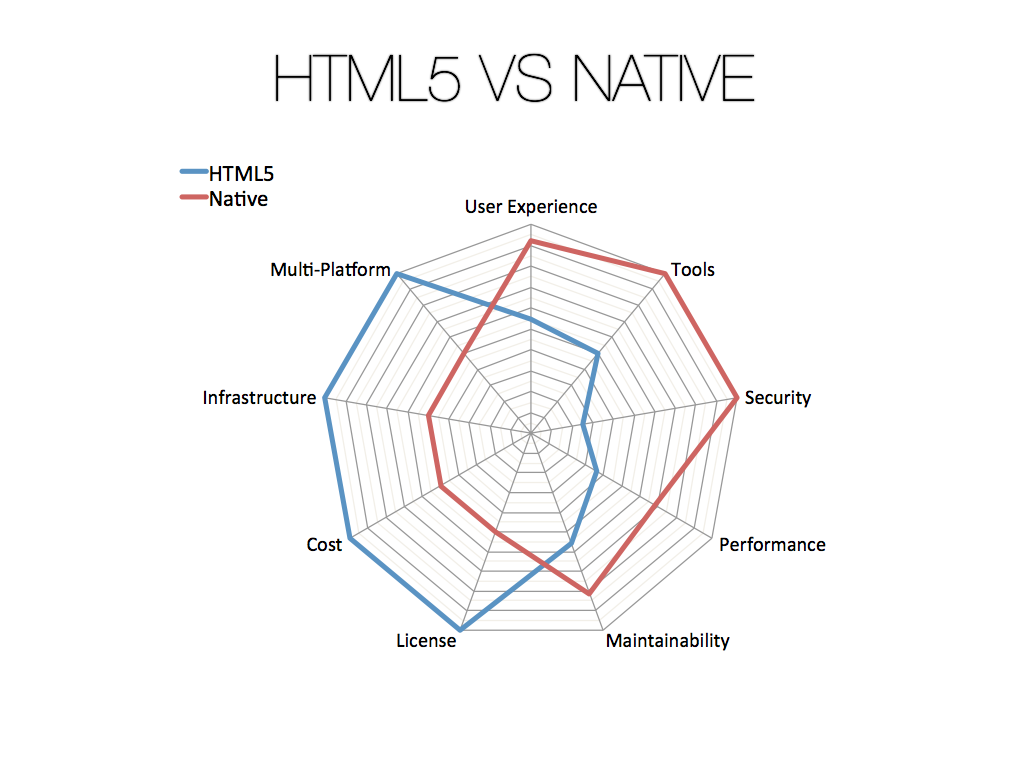
\includegraphics[scale=0.4]{html5_mobile.png}
\caption{HTML5 vs NATIVE }
\end{figure}

Các tính năng chính hỗ trợ cho các thiết bị di động

\textbf{Hỗ trợ offline:}

Các AppCache và cơ sở dữ liệu làm cho nó có thể cho các nhà phát triển di động để lưu trữ những thứ trên các thiết bị và gián đoạn trong kết nối sẽ không ảnh hưởng đến khả năng cho một người nào đó để có được công việc của họ thực hiện.

Hỗ trợ offline giúp trình duyệt bộ nhớ cache các trang tĩnh. Họ phụ thuộc nhiều vào HTTP tiêu đề phản ứng gửi bởi máy chủ web để lấy HTML, CSS và đa phương tiện cần thiết để làm cho trang web. Nếu tất cả mọi thứ cần thiết để làm được lưu trữ, sau đó sẽ được tải nhanh chóng, nhưng ngay cả khi một mục không được lưu trữ sau đó tất cả mọi thứ chậm lại đáng kể.

Để cung cấp hỗ trợ offline, một biểu hiện tập tin bộ nhớ cache phải được tạo ra để xác định ứng dụng của tài nguyên ẩn-tức là các trang của nó, hình ảnh, và các tập tin khác cần thiết để chạy offline. Thông thường, các biểu hiện cũng có một ý kiến được thay đổi khi có các nguồn tài nguyên thay đổi, khiến trình duyệt để làm mới bộ nhớ cache.

\textbf{Canvas:}

Các trang web có thể đánh dấu ra một không gian trên một trang mà hình ảnh tương tác, biểu đồ và đồ thị, các thành phần trò chơi, và tưởng tượng khác có thể được rút ra trực tiếp bằng mã lập trình và tương tác người dùng - không có flash hoặc các plug-in được yêu cầu.

\textbf{Video và hỗ trợ truyền audio:}

Phát triển đang trong giai đoạn rất sớm và phải gián đoạn định dạng, nhưng các trang web như YouTube và Pandora một ngày có thể bỏ qua flash hoàn toàn và mang lại chức năng phát lại theo thời gian và các tính năng hơn nữa.

\textbf{GeoLocation API:}

Điều này thực sự không phải một phần của HTML5, nhưng là một đặc điểm kỹ thuật riêng biệt. Các định vị API cho phép bạn chia sẻ vị trí của bạn với các trang web đáng tin cậy. (Điều này thực sự là vị trí địa lý của thiết bị hoặc kết nối internet của bạn, quyết định dựa trên sự kết hợp của GPS, gia tốc, điện thoại di động tháp tam giác, và ISP hồ sơ địa chỉ.) Các vĩ độ và kinh độ có sẵn để JavaScript trên trang web, mà trong lần lượt có thể gửi lại cho máy chủ web từ xa và cho bạn nhận biết vị trí nội dung như các doanh nghiệp địa phương hoặc hiển thị vị trí của bạn trên bản đồ.
Sau đây là nổi bật API cho một định vị.
 navigator.geolocation.getCurrentPosition(successCallback, errorCallback, options);
Định vị là một đối tượng mà là một phần của đối tượng Navigator. Nó sử dụng phương thức getCurrentPosition(). Tìm kiếm vị trí là một hoạt động không đồng bộ vì nó đòi hỏi sự cho phép của người dùng để truy cập. Do đó chức năng gọi lại cho sự thành công và thất bại là bắt buộc.

\textbf{Form nâng cao:}

Ngay cả điều đơn giản như những cải tiến trong HTML5 cho các hình thức có thể làm cho cuộc sống dễ dàng hơn cho các ứng dụng điện thoại di động. Các lĩnh vực có thể được xác nhận bởi các trình duyệt được cải tiến cho các thiết bị di động. Các chi tiết mà có thể được xử lý bởi các trình duyệt có nghĩa là ít thời gian tải JavaScript mã và các chuyến đi vòng ít đến máy chủ nếu xác nhận có thể được tìm thấy trước khi biểu mẫu được đăng.

\subsection{Kiến thức về JavaScript}
\subsubsection{Tổng quan về JavaScript}
JavaScript là một ngôn ngữ lập trình. Là một phần của các trình duyệt web, cho phép triển khai kịch bản phía máy khách để tương tác với người sử dụng, kiểm soát trình duyệt, giao tiếp không đồng bộ, và làm thay đổi nội dung được hiển thị. Nó cũng đã trở nên phổ biến trong lập trình phía máy chủ, phát triển trò chơi và tạo ra các ứng dụng máy tính.

JavaScript có cú pháp bị ảnh hưởng bởi C cũng như có nhiều quy ước đặt tên từ Java, nhưng chúng không liên quan và có ngữ nghĩa rất khác nhau. Đây là một mô hình đa ngôn ngữ, hỗ trợ hướng đối tượng, bắt buộc, và mang phong cách lập trình chức năng.
 
Là ngôn ngữ thông dịch, đoạn mã JavaScript được nhúng hoặc tích hợp vào file HTML. Khi trang web được tải trong trình duyệt hỗ trợ JavaScript, Trình duyệt sẽ thông dịch và thực hiện các lệnh JavaScript.

JavaScript được sử dụng nhằm bổ sung sự tương tác cho các trang HTML như:

\quad - JavaScript có thể đáp ứng các sự kiện như tải hay loại bỏ các form. Khả năng này cho phép JavaScript trở thành một ngôn ngữ script động.

\quad - JavaScript có thể được sử dụng để xác nhận dữ liệu người dùng nhập vào trước khi nó được chuyển đến server.

\quad - Sử dụng JavaScript có thể giúp website của bạn tương tác với người dùng 1 cách uyển chuyển hơn.

\quad - Tùy biến trình duyệt...

Tóm lại, JavaScript giống như phần hồn của một trang web, giúp người sử dụng có thể tương tác một cách tiện lợi hơn bên cạnh phần xác HTML.


\subsubsection{Cấu trúc và các thành phần trong JavaScript}
\textbf{Các kiểu dữ liệu}

Một biến trong JavaScript các kiểu dữ liệu. Ba kiểu thông thường là: boolean, number, string. Hai kiểu phức tạp là: array và object. Và cuối cùng là kiểu đặc biệt: NULL.

\textbf{Biến}

Biến trong JavaScript đuợc khai báo bởi từ khóa “var” và theo sau là tên của biến. Tên biến phân biệt chữ hoa và chữ thường. Tên biến phải bắt dầu bằng một chữ cái hay một dấu gạch nối, theo sau là các chữ cái, chữ số hay là dấu gạch nối. Thậm chí ta cũng không cần khai báo từ khóa "var" nhưng điều này không được khuyến cáo sử dụng.
  
Ví dụ:  
\begin{lstlisting}
	var name1="John";
	var name2="John";
	name3="John";
\end{lstlisting}


\textbf{Cấu trúc rẽ nhánh}

Các câu lệnh này cho phép chúng ta phân biệt các khối mã lệnh mà sẽ được thực thi chỉ khi gặp phải các điệu kiện nào đó. JavaScript cung cấp hai cấu trúc lệnh điều kiện. Đầu tiên là if...else, cho phép chúng ta có thể kiểm tra một số lượng các biểu thức và thực thi các câu lệnh theo giá trị của chúng. Nếu chúng ta mong muốn kiểm tra một biểu thức đơn lẻ với một số lượng các giá trị, JavaScript cũng cung cấp một cấu trúc switch...case mà có thể làm đơn giản hoá đi phép toán này.
 
Câu lệnh “if… else…”: Câu lệnh if là một trong những đặc tính quan trọng nhất của mỗi  ngôn ngữ lập trình. Nó cho phép thực thi chọn lựa các dòng mã lệnh chỉ khi thoả mãn các điều kiện cụ thể.
  
Câu lệnh “switch… case…”: được sử dụng khi một biến riêng rẽ đang được kiểm tra so với các giá trị khác.Ví dụ:

\begin{lstlisting}
switch (country) { 
       case "ca": 
          alert ("Canada"); 
          break; 
       case "uk": 
         alert ("the United Kingdom"); 
          break; 
       default:  
          alert ("the United States"); 
}
\end{lstlisting}


Khi câu lệnh switch thực hiện kiểm tra giá trị của biến country và so sánh nó với mỗi một trong các giá trị trong các mệnh đề case. Khi một giá trị thích hợp được tìm thấy, các câu lệnh kết hợp với case được thực hiện cho đến khi gặp câu lệnh break. Còn nếu không tìm ra được giá trị thích hợp nào thì câu lệnh default sẽ được thực hiện.

\textbf{Vòng lặp}  

Các vòng lặp chính là các phương tiện của việc thực thi một khối mã lệnh trong một số lần cho trước hay là cho đến khi gặp phải một điều kiện nhất định. 
JavaScript có hai loại vòng lặp: vòng lặp while kiểm tra điều kiện trước hay là sau mỗi bước tính lặp đi lặp lại và thực hiện lặp lại chỉ khi điều kiện là đúng. Một kiểu lặp khác là for, trong trường hợp này, số lượng bước tính lặp đi lặp lại được qui định trước khi lặp lần đầu và không thể bị thay đổi.  
Vòng lặp while: là câu lệnh lặp đơn giản nhất. Cú pháp tương tự như câu lệnh if:

\begin{lstlisting}
	while (i < 10) {
	    alert(i);
	    i = i + 1;
	}
\end{lstlisting} 

Vòng lặp for: Cấu trúc của vòng lặp for là khá phức tạp hơn mặc dù vòng lặp for thường tiện lợi hơn vòng lặp while:

\begin{lstlisting}
	for (var i = 1; i < 10; i++) {
	    alert(i);
	}
\end{lstlisting}


\textbf{Hàm}

Tên hàm có thể được gọi tại bất kỳ đâu trong chương trình, cho phép các đoạn mã thể hiện bởi tên của nó được thực hiện lặp lại khi cần thiết. Tạo một hàm JavaScript là một quá trình đơn giản. Bạn có thể tạo một hàm tại bất kỳ nơi nào trong chương trình JavaScript. Tuy nhiên, cho mục đích tổ chức bạn có thể thấy rằng sự thuận lợi khi đặt tất cả các hàm được dự định sẽ sử dụng trong script tại đầu mỗi file script. Một phương thức khác cho việc tổ chức hàm mà có thể giảm đi sự dư thừa đáng kể và tăng việc sử dụng lại là đặt các hàm trong những file riêng rẽ (được xem như là một thư viện).
    
Ví dụ khai báo một hàm sau:  

\begin{lstlisting}
	var add = function (a, b) { return a + b; }; 
\end{lstlisting}

Ta có thể lưu các hàm như giá trị của một biến, và gọi một hàm bằng cách sử dụng biến này và một cặp dấu ngoặc đơn. Điều này cũng được gọi là gọi hàm.

\subsubsection{DOM}

Document Object Model là một cách để thao tác các cấu trúc và phong cách của một trang HTML. Nó đại diện cho phần bên trong của các trang như cách trình duyệt nhìn thấy nó, và cho phép các nhà phát triển để thay đổi nó với JavaScript.

HTML là một cấu trúc XML giống như trong các yếu tố tạo thành một cấu trúc của nút cha với nút con, như các nhánh của một cây. Có một phần tử gốc (<html>) với các nhánh như <head> và <body>. Vì lý do này, DOM cũng được gọi là cây DOM.

Sửa đổi DOM, bằng cách chọn một phần tử và thay đổi một thuộc tính về nó, là một việc thực hiện thường xuyên trong JavaScript. Để truy cập vào DOM từ JavaScript, sử dụng các đối tượng document. Nó được cung cấp bởi các trình duyệt và cho phép mã trên trang để tương tác với các nội dung.

Điều đầu tiên phải biết là làm thế nào để có được một phần tử. Có một số cách để làm việc đó, và các trình duyệt hỗ trợ những người khác nhau. Cách hay sử dụng nhất là chọn đối tượng theo ID riêng biệt của đối tượng đó.

\begin{lstlisting}
	var pageHeader = document.getElementById('page-header');
\end{lstlisting}

Các đối tượng có “id=pageHeader” sau đó có thể được thao tác. Các thuộc tính của nó có thể được thay đổi, và mã khác có thể được khai báo để xử lý các yếu tố được click hoặc hover.


\subsubsection{Sự kiện(event)}

Trong trình duyệt nhất đang hướng sự kiện và viết các ứng dụng tương tác trong JavaScript thường là về chờ đợi và phản ứng với các sự kiện để thay đổi hành vi của trình duyệt một cách nào đó. Sự kiện xảy ra khi tải trang, khi có tương tác người dùng (click, hover, change…). Dưới đây là một nhóm trong những điều cần thiết để lắng nghe cho một sự kiện, chức năng gọi lại, một phần tử gọi đến một sự kiện:
 
\begin{lstlisting}
	var handleClick = function (event) { // do something! }; 
	var button = document.querySelector('#big-button'); 
	button.addEventListener('click', handleClick);
\end{lstlisting}


addEventListener() là một phương thức được tìm thấy trên tất cả các yếu tố DOM. Ở đây nó được gọi là trên một phần tử được lưu trong biến button. Tham số đầu tiên là một chuỗi - tên của sự kiện để lắng nghe. Dưới đây là đó là click – sự kiện nhấp chuột. Thứ hai là chức năng callback – ở đây gọi hàm handleClick.
Có nhiều loại sự kiện mà JavaScript hỗ trợ và được sử dụng phổ biến như onblur, onchange, onsubmit, onkeydown, onmouseover…

\subsubsection{AJAX}

Để có được nội dung mới của trang web, ta phải di chuyển từ trang này sang trang kế tiếp. Nhưng như các nhà phát triển có nhiều tham vọng hơn với các trang web, cố gắng để xây dựng tương tác thật nhất, và rõ ràng là cần thiết để có thể là một cách để tải nội dung mới vào một trang mà không cần tải lại đầy đủ.

Để tải nội dung mới cho một trang, như nội dung mới trên một trang web hoặc thông báo có email mới, một công cụ được gọi là một yêu cầu XML HTTP (XHR) được sử dụng. Các ứng dụng web mà làm điều này còn được gọi là các ứng dụng AJAX. AJAX là viết tắt của Asynchronous JavaScript And XML.

\begin{figure}[!htb] 
\centering
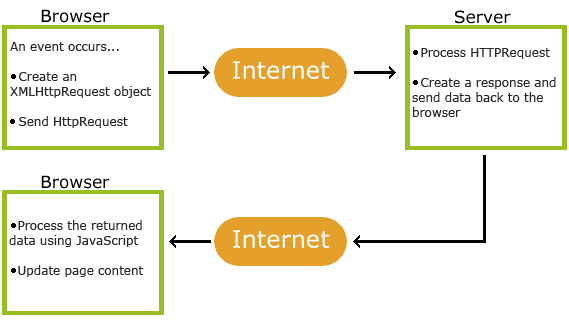
\includegraphics[scale=0.8]{ajax.png}
\caption{Công nghệ AJAX}
\end{figure}

Ví dụ về một XMLHttpRequest:

\begin{lstlisting}
var req = new XMLHttpRequest(); 
req.onload = function (event) { . . . }; 
req.open('get', 'some-file.txt', true); 
req.send(); 
\end{lstlisting}

Điều đầu tiên là tạo mới một XMLHttpRequest bằng cách sử dụng từ khóa “new”, và gọi XMLHttpRequest như một hàm.
Sau đó, chỉ định một hàm callback, để được gọi khi dữ liệu được nạp. Nó được thông qua thông tin về sự kiện này như là đối số đầu tiên.

Sau đó, xác định như thế nào để có được những dữ liệu bằng cách sử dụng req.open. Tham số đầu tiên là phương pháp HTTP (GET, POST, PUT vv). Tiếp theo là các URL để lấy từ dữ liệu (tương tự như href thuộc tính của một liên kết).

Tham số thứ ba là một biến boolean xác định xem yêu cầu là không đồng bộ - ở đây là true, vì vậy XMLHttpRequest được gửi và sau đó thực thi mã vẫn tiếp tục cho đến khi một phản hồi từ máy chủ làm cho hàm onload được gọi lại.

Giá trị mặc định tham số không đồng bộ là false, tức là thực hiện của mã này sẽ tạm dừng tại dòng này cho đến khi dữ liệu được lấy ra và yêu cầu được gọi là đồng bộ. XMLHttpRequests đồng bộ không được sử dụng thường xuyên như là một yêu cầu tới một máy chủ được gửi đi liên tục.

Trên dòng cuối cùng chúng em cho trình duyệt để gửi đi các yêu cầu dữ liệu.

\subsubsection{LocalStorage}

\textbf{LocalStorage}
Khi xây dựng các ứng dụng JavaScript phức tạp chạy trong trình duyệt của người dùng nó rất hữu ích để có thể lưu trữ thông tin trong trình duyệt, do đó các thông tin có thể được chia sẻ trên các trang khác nhau và các phiên duyệt web.
Trong thời gian qua điều này sẽ chỉ thực hiện được với các tập tin cookie - tập tin văn bản được lưu vào máy tính của người dùng - nhưng cách quản lý những việc này với JavaScript là không tốt. Bây giờ có một công nghệ mới được gọi là LocalStorage mà không một điều tương tự, nhưng với một giao diện dễ dàng hơn để sử dụng.

Không giống như các tập tin cookie, Local Storage chỉ có thể được đọc phía máy khách - đó là, bởi trình duyệt và JavaScript. Nếu muốn chia sẻ một số dữ liệu với máy chủ, các tập tin cookie có thể là một lựa chọn tốt hơn.
Để lưu dữ liệu, sử dụng localStorage.getItem:
localStorage.setItem('name', 'tom'); 
Đối số đầu tiên xác định tên sẽ sử dụng để lấy dữ liệu ra. Đối số thứ hai là các dữ liệu ta muốn lưu trữ.
Nhận được trở lại một lần nữa là rất đơn giản - chỉ cần gọi phương thức localStorage.getItem
var name = localStorage.getItem('name');


\textbf{SessionStorage}

Chức năng tương tự như LocalStorage, tuy nhiên dữ liệu sẽ được xóa khi thoát khỏi trình duyệt, hay ứng dụng do đó không gây tốn kém tài nguyên và bảo mật dữ liệu hơn.


\subsubsection{Thư viện Jquery}

jQuery là thư viện JavaScript đa trình duyệt được thiết kế để đơn giản hóa lập trình phía máy người dùng của HTML. jQuery được làm cho việc di chuyển một tài liệu dễ dàng hơn, chọn các yếu tố DOM, tạo ra hiệu ứng, xử lý sự kiện, và phát triển ứng dụng AJAX.

\textbf{Cách sử dụng jQuery}

jQuery thay đổi cách chọn một đối tượng DOM, khiến cho việc thao tác với đối tượng trở nên đơn giản hơn. Thay vì sử dụng phương thức getElementsById(id) của JavaScript thuần, jQuery thu gọn lại bằng cách viết \textdollar(id).

Ví dụ:

\begin{lstlisting}
//trong JavaScript
document.getElementsById("header")[0].innerHTML = "Change the page.";
//trong Jquery
$("#header").html("Change the page.");
\end{lstlisting}

\textbf{AJAX}

jQuery có thể thực hiện trình duyệt độc lập truy vấn AJAX sử dụng cú pháp \textdollar.ajax đơn giản hơn và phương pháp liên kết để tải và thao tác dữ liệu từ xa.

\begin{lstlisting}
$.ajax ( {
   type : "POST" ,
   url : "example.php" ,
   data : "name=John&location=Boston"
 } ) . done ( function ( msg ) {
   alert ( "Data Saved: " + msg ) ;
 } ) . fail ( function ( xmlHttpRequest , statusText , errorThrown ) {
   alert (
     "Your form submission failed. \n \n "
       + "XML Http Request: " + JSON. stringify ( xmlHttpRequest )
       + ", \n Status Text: " + statusText
       + ", \n Error Thrown: " + errorThrown ) ;
 } ) ;
\end{lstlisting}

\subsubsection{Thư viện Jquery Mobile}

jQuery Mobile là một framework web được tối ưu cho màn hình cảm ứng (được gọi là một thư viện JavaScript hoặc một framework di động) hiện đang được phát triển bởi nhóm dự án jQuery. Sự phát triển tập trung vào việc tạo ra một khuôn khổ tương thích với một loạt các điện thoại thông minh và máy tính bảng. jQuery Mobile là tương thích với các framework ứng dụng di động và các nền tảng khác như như PhoneGap, Worklight và nhiều hơn nữa.

Tính năng:

\quad - Tương thích với tất cả các nền tảng di động lớn cũng như tất cả các trình duyệt máy tính để bàn lớn, bao gồm iOS, Android, Blackberry, WebOS, Symbian, Windows Phone và nhiều hơn nữa.

\quad - Được xây dựng trên lõi jQuery vì vậy nó khá quen thuộc cho những người đã biết cú pháp jQuery.

\quad - Cho phép tạo ra các chủ đề, giao diện tùy chỉnh.

\quad - Hạn chế phụ thuộc và nhẹ để tối ưu hóa tốc độ.

\quad - Codebase cơ bản giống nhau sẽ tự động quy mô cho bất kỳ màn hình.

\quad - Cấu hình hướng HTML5 để đặt ra các trang web có đoạn mã tối thiểu.

\quad - Hướng Ajax hỗ trợ với quá trình hiệu ứng chuyển đổi trang, cung cấp khả năng làm sạch các URL thông qua pushState.

\quad - Vật dụng giao diện người dùng tối ưu hóa cảm ứng.

Một trang web sử dụng jQuery Mobile thường có một "header", một "footer" và "content”. Một file HTML có thể chứa nhiều hơn một yếu tố "page" do đó nhiều hơn một "trang web". Bằng cách này, nó chỉ là cần thiết để tải một tập tin bao gồm nhiều trang. Một trang có thể liên kết đến một trang khác trong cùng một tập tin bằng cách sử dụng "\#" cùng với id của nó (ví dụ: href = “\#second”).

Ngoài ra, jQuery Mobile còn có các thuộc tính “data-” với các chức năng khác nhau:

\quad -vData-role: Xác định vai trò của các yếu tố, như tiêu đề, nội dung, footer,…

\quad - Data-position: xác định xem thành phần sẽ được cố định, trong trường hợp này nó sẽ làm cho đối tượng ở phía trên (đối với header) hoặc dưới (đối với footer).

\quad - Data-transition: mô tả quá trình chuyển đổi để sử dụng khi tải trang mới, có thể được thiết lập để: slide, slideUp, slideDown, pop, slide hoặc fade…

\quad - Data-theme: mô tả chủ đề thiết kế để sử dụng cho các yếu tố bên trong container, có thể được thiết lập để chọn các giao diện có sẵn.

Ví dụ:

\begin{lstlisting}
<div data-role="header" data-theme="b"> 
	<h1>Page Title</h1> 
</div>
\end{lstlisting}

Đoạn mã trên đã đặt thẻ “div” ở vị trí đầu trang (header) và qua định giao diện có sẵn “b” của jQuery Mobile.

\subsubsection{Ghi chú quan trọng cần nhớ khi sử dụng JavaScript}

Lệnh Javascript phân biệt chữ in hoa và chữ thường.

Mội câu lệnh Javascript đều kết thúc bằng dấu chấm phẩy “;”.

Các điều kiện phải được khai báo trong cặp dấu ngoặc đơn ().

Khi sử dụng lệnh điều khiển, nếu sử dụng nhiều hơn 1 lệnh, phải sử dụng cặp dấu ngoặc nhọn {}

Javascript sử dụng dấu chấm “.” để tham chiếu đến 1 phương thức hay thuộc tính của đối tượng 

\subsection{Hệ thống quản lý học tập Moodle}

Moodle (viết tắt của Modular Object-Oriented Dynamic Learning Environment) là một nền tảng phần mềm miễn phí về e-learning, còn được gọi là một hệ thống quản lý học tập (Learning Management System). Moodle được phát triển để giúp các nhà giáo dục tạo ra các khóa học trực tuyến tập trung vào sự tương tác và xây dựng hợp tác nội dung, và đang trong quá trình tiến hóa liên tục.

Moodle cho phép tạo các khóa học trên Internet hay các trang web học tập trực tuyến. Moodle được thiết kế dựa trên module nên ta có thể chỉnh sửa giao diện bằng các theme có sẵn hoặc thêm một theme mới cho riêng mình.

\begin{figure}[!htb] 
\centering
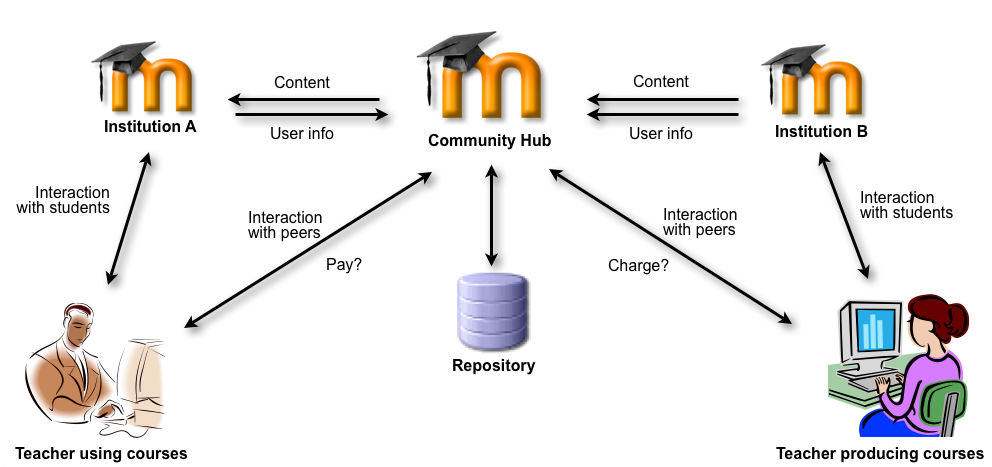
\includegraphics[scale=0.4]{moodle_system.png}
\caption{Moodle}
\end{figure}

Moodle hoàn toàn phù hợp với nhiều cấp học và loại hình đào tạo như phổ thông, đại học hoặc cao đẳng, chính quy hoặc không chính quy và trong các tổ chức, công ty.
Moodle được phát triển dựa trên PHP, có thể triển khai trên một nhóm nhỏ hoặc trên cả các cụm đại học lớn. Vì thế, Moodle có thể giúp chúng ta tiết kiệm rất nhiều khi triển khai một hệ thống e-Learning.
Một số tính năng điển hình của Moodle là:

\quad - Trình chuyển nhượng

\quad - Diễn đàn thảo luận

\quad - Các tập tin tải về

\quad - Phân loại

\quad - Tin nhắn tức thời moodle

\quad - Lịch trực tuyến

\quad - Tin tức trực tuyến và thông báo

\quad - Bài kiểm tra trực tuyến

\quad - Wiki

Phát triển có thể mở rộng xây dựng mô-đun của Moodle bằng cách tạo bổ sung cho chức năng mới cụ thể. Cơ sở hạ tầng của Moodle hỗ trợ nhiều loại plug-in :

\quad - Hoạt động (bao gồm cả chữ và các trò chơi toán học)

\quad - Các loại tài nguyên

\quad - Dạng câu hỏi (nhiều lựa chọn, đúng và sai, điền vào chỗ trống, vv)

\quad - Kiểu trường dữ liệu (đối với hoạt động cơ sở dữ liệu)

\quad - Giao diện đồ họa

\quad - Phương pháp xác thực (có thể yêu cầu tên người dùng và mật khẩu truy cập)

\quad - Phương pháp tuyển sinh

\quad - Bộ lọc nội dung

\subsection{Bộ phát triển ứng dụng Cordova (PhoneGap)}

Cordova (PhoneGap) là một khuôn khổ phát triển điện thoại di động. Nó cho phép phần mềm lập trình để xây dựng các ứng dụng cho các thiết bị di động sử dụng JavaScript, HTML5, và CSS3 thay vì ngôn ngữ thiết bị cụ thể như Objective-C. Các ứng dụng kết quả là lai, có nghĩa là họ không phải là thực sự bản địa (vì tất cả việc xử lý layout được thực hiện thông qua webview thay vì nguồn gốc khung giao diện của nền tảng), cũng không hoàn toàn dựa trên web (vì chúng không chỉ là các ứng dụng web, nhưng được đóng gói như các ứng dụng để phân phối và được tiếp cận với thiết bị có nguồn gốc API ).

Lõi của ứng dụng PhoneGap sử dụng HTML5 và CSS3 để tạo giao diện, và JavaScript cho các phương thức xử lý. Mặc dù HTML5 hiện nay cung cấp quyền truy cập vào phần cứng cơ bản như gia tốc, camera và GPS, trình duyệt hỗ trợ để truy cập thiết bị nền HTML5 dựa trên là không phù hợp trên các trình duyệt di động, đặc biệt là phiên bản cũ của Android. Để khắc phục những hạn chế, framework Cordova nhúng mã HTML5 bên trong một WebView bản địa trên thiết bị, sử dụng một giao diện chức năng ngoài để truy cập vào các nguồn tài nguyên tự nhiên của thiết bị.

\begin{figure}[!htb] 
\centering
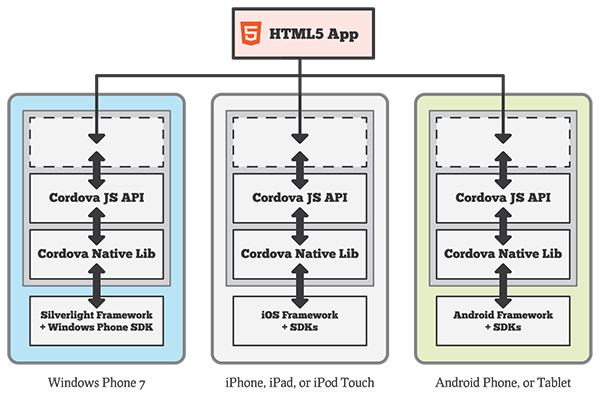
\includegraphics[scale=0.6]{html5app.png}
\caption{Ứng dụng HTML5}
\end{figure}

Cordova cũng có thể được mở rộng với nguồn gốc của các plug-in cho phép các nhà phát triển thêm các chức năng có thể được gọi từ JavaScript, cho phép giao tiếp trực tiếp giữa các lớp bản địa và các trang HTML5. Cordova bao gồm bổ sung cơ bản cho phép truy cập vào gia tốc của thiết bị, camera, microphone, la bàn, hệ thống tập tin, và nhiều hơn nữa.

Tuy nhiên, việc sử dụng công nghệ web dựa trên dẫn nhiều ứng dụng Cordova để chạy chậm hơn so với các ứng dụng bản địa với chức năng tương tự. Adobe Systems cảnh báo rằng các ứng dụng được xây dựng sử dụng Cordova có thể bị từ chối bởi của Apple là quá chậm hoặc không cảm thấy "bản địa" đủ (có sự xuất hiện và chức năng phù hợp với những gì người dùng đã mong đợi trên nền tảng này).

\subsection{Nền tảng ứng dụng di động Worklight}

IBM Worklight cung cấp một nền tảng ứng dụng di động cao cấp, toàn diện và mở, có thể giúp phát triển, chạy và quản lý có hiệu quả các ứng dụng HTML5, lai và nguyên gốc, bằng cách sử dụng các công nghệ và các công cụ dựa trên các tiêu chuẩn, phần mềm trung gian tối ưu hóa cho di động, một loạt các cơ chế bảo mật và các khả năng phân tích và quản lý tích hợp.

\begin{figure}[!htb] 
\centering
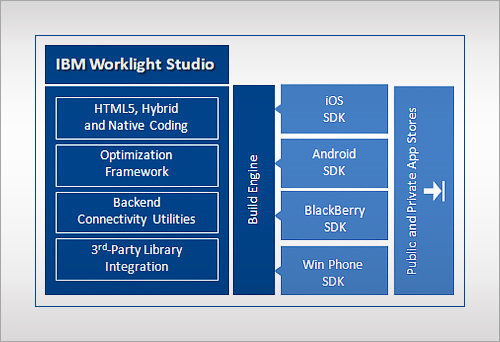
\includegraphics[scale=0.6]{worklight_eco.png}
\caption{Nền tảng ứng dụng di động Worklight}
\end{figure}

Worklight giúp xây dựng các ứng dụng lai (hybrid), bổ sung những khiếm khuyết của ứng dụng nền web như không can thiệp sâu vào thiết bị hay không khởi chạy được các thành phần đa phương tiện bằng những phương thức của ứng dụng nguyên bản (native).

Đề tài được ứng dụng trên phiên bản Worklight 6 của IBM.

\subsection{Truyền thông qua Web services}
\subsubsection{Tổng quan về Web services}

Web services là kiến trúc hỗ trợ khả năng tương tác của các ứng dụng trên các máy tính khác nhau thông qua mạng Internet với giao diện chung và sự gắn kết được mô tả bằng XML và truy xuất thông qua web dùng URL.

Lợi điểm của Web services là chi phí phát triển thấp, dễ bảo trì, cho phép Client và Server tương tác được với nhau trong những môi trường khác nhau.

Web services là một dịch vụ cung cấp cơ chế triệu gọi các đối tượng từ xa thông qua giao thức HTTP cùng với cơ chế truyền tải định dạng đối tượng theo công nghệ XML. Chính vì sử dụng giao thức HTTP của Web nên giờ đây các lời gọi trở nên đơn giản và thông qua được các rào cản về tường lửa. Để đảm bảo điều này, một giao thức mới là SOAP (Simple Object Access Protocol) ra đời để hỗ trợ cho Web services.  

\textbf{SOAP – Simple Object Access Protocol}

SOAP được định nghĩa dựa trên giao thức chuẩn HTTP, SOAP cho phép dữ liệu chuyển đi bằng HTTP và định dạng theo chuẩn XML. Các lời gọi hàm tham số truyền hàm, dữ liệu trả về từ hàm, tất cả đều được chuyển sang dạng XML và có thể dễ dàng xử lý bởi tất cả các ngôn ngữ. Một thế mạnh khác đó là nếu các đối tượng phân tán xây dựng trên mô hình Web services sẽ có thể triệu gọi lẫn nhau, bất chấp đối tượng đó được viết trên ngôn ngữ Java của Sun hay .NET của Microsoft.
  
Hiện tại, SOAP được coi là một sự thay đổi lớn kể từ khi COM, RMI, CORBA ra đời.

\subsubsection{Đặc điểm web services}

\textbf{Độc lập ngôn ngữ:}

Web services được truy xuất thông qua Web bằng cách dùng URL.

Web services liên lạc với thế giới bên ngoài dùng thông điệp XML gửi trực tiếp qua các giao thức Web.

Web services được đăng ký tại nơi chung, và được đặc tả tất cả các chức năng.

\textbf{Chi phí phát triển thấp, dễ bảo trì.}

Dịch vụ Web cho phép client và server tương tác được với nhau ngay cả trong những môi trường khác nhau. Ví dụ, đặt Web server cho ứng dụng trên một máy chủ chạy hệ điều hành Linux trong khi người dùng sử dụng máy tính chạy hệ điều hành Windows, ứng dụng vẫn có thể chạy và xử lý bình thường mà không cần thêm yêu cầu đặc biệt để tương thích giữa hai hệ điều hành này.

Phần lớn kĩ thuật của Dịch vụ Web được xây dựng dựa trên mã nguồn mở và được phát triển từ các chuẩn đã được công nhận, ví dụ như XML.

Một Dịch vụ Web bao gồm có nhiều mô-đun và có thể công bố lên mạng Internet.

Là sự kết hợp của việc phát triển theo hướng từng thành phần với những lĩnh vực cụ thể và cơ sở hạ tầng Web, đưa ra những lợi ích cho cả doanh nghiệp, khách hàng, những nhà cung cấp khác và cả những cá nhân thông qua mạng Internet.

Một ứng dụng khi được triển khai sẽ hoạt động theo mô hình client-server. Nó có thể được triển khai bởi một phần mềm ứng dụng phía server ví dụ như PHP, Oracle Application server hay Microsoft.Net…

Ngày nay dịch vụ Web đang rất phát triển, những lĩnh vực trong cuộc sống có thể áp dụng và tích hợp dịch vụ Web là khá rộng lớn như dịch vụ chọn lọc và phân loại tin tức (hệ thống thư viện có kết nối đến web portal để tìm kiếm các thông tin cần thiết); ứng dụng cho các dịch vụ du lịch (cung cấp giá vé, thông tin về địa điểm…), các đại lý bán hàng qua mạng, thông tin thương mại như giá cả, tỷ giá hối đoái, đấu giá qua mạng…hay dịch vụ giao dịch trực tuyến (cho cả B2B và B2C) như đặt vé máy bay, thông tin thuê xe…

Các ứng dụng có tích hợp dịch vụ Web đã không còn là xa lạ, đặc biệt trong điều kiện thương mại điện tử đang bùng nổ và phát triển không ngừng cùng với sự lớn mạnh của Internet. Bất kì một lĩnh vực nào trong cuộc sống cũng có thể tích hợp với dịch vụ Web, đây là cách thức kinh doanh và làm việc có hiệu quả bởi thời đại ngày nay là thời đại của truyền thông và trao đổi thông tin qua mạng. Do vậy, việc phát triển và tích hợp các ứng dụng với dịch vụ Web đang được quan tâm phát triển là điều hoàn toàn dễ hiểu.

\section{Khảo sát}

Nhìn chung lĩnh vực E-learning trên tablet cũng khá nổi trong những năm gần đây, khi mà giá thành chiếc tablet ngày càng rẻ, hơn nữa tablet sẽ dễ dàng sử dụng hơn là laptop hay desktop. Một trong những phần mềm học tiếng Anh mà chúng em đã khảo sát sau đây khá điển hình. Phần mềm luyện nghe tiếng anh thường chỉ chạy trên một nền tảng nhất định, trong trường hợp này là viết bằng Java chạy trên hệ điều hành Android. Trong khi đó phần mềm mà chúng em viết bằng JavaScript, và chỉnh cần tinh chỉnh một chút là có thể chạy cả trên Android hay iOS.
\subsection{IELTS Listening}

\begin{figure}[!htb] 
\centering
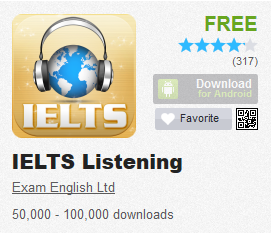
\includegraphics[scale=0.8]{iel.png}
\caption{Chương trình IELTS Listening trên Android}
\end{figure}

Chương trình luyện nghe IELTS miễn phí chạy trên Android với lượt download là 50,000-100,000:

Đường dẫn đến website \url{http://www.appszoom.com/android_applications/education/ielts-listening_hddku.html}

\begin{figure}[!htb] 
\centering
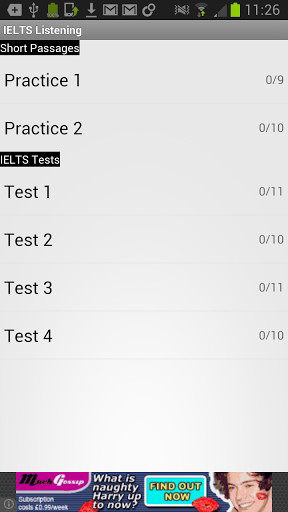
\includegraphics[scale=0.4]{iel1.png}

\caption{Màn hình chọn bài học của chương trình}
\end{figure}

\begin{figure}[!h] 
\centering
\subfigure[Màn hình trả lời trắc nghiệm]{
   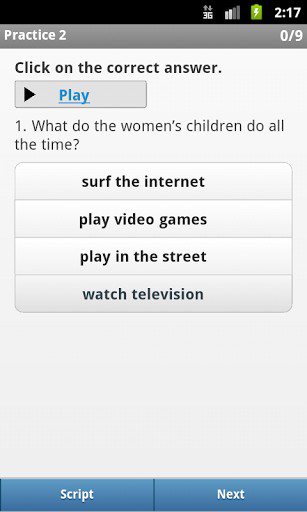
\includegraphics[width=0.30\textwidth] {iel2.png}
   \label{fig:MultipleChoices}}
\subfigure[Màn hình điền từ vào chỗ trống]{
   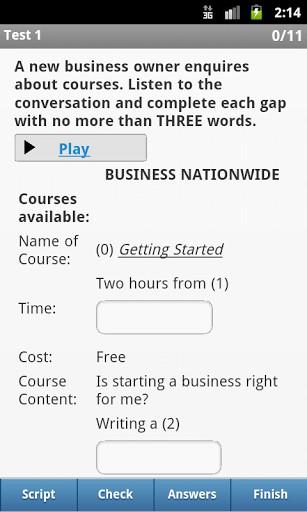
\includegraphics[width=0.30\textwidth] {iel3.png}
   \label{fig:Fillblank}}

\caption{Màn hình chính của chương trình }
\end{figure}




\subsection{English Ant plus}

English Ant plus (Bản office): Phần mềm học tiếng anh trên android

Giao diện đơn giản, dễ nhìn.

\begin{figure}[!htb] 
\centering
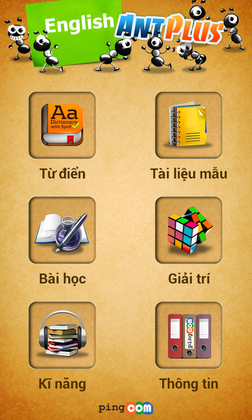
\includegraphics[scale=0.8]{hinh1_menu.png}
\caption{Màn hình menu của chương trình}
\end{figure}

Phần mềm có các chức năng chính như sau:

\quad 1. Từ điển

Chức năng Từ điển cũng tương tự như các từ điển thông dụng.


Khi đánh một từ thì 1 danh sách từ được đề nghị xổ xuống.

Có từ điển chuyên ngành về kỹ thuật và kinh tế.

\quad 2. Tài liệu mẫu

Có một thư viện mẫu về Thư giao dịch, Sơ yếu lý lịch và Hợp đồng mẫu bằng Tiếng Anh.

Mỗi một mục phân ra làm nhiều lĩnh vực, ngành nghề khác thuận tiện trong việc tìm kiếm.

Đa số các lĩnh vực phổ biến nó đều có như: thư giao dịch trong ngân hàng, mua bán, các hợp đồng làm ăn…

\quad 3. Bài học

Chứa các bài học về ngữ pháp, từ vựng.

Có hầu hết các chủ đề phổ biến.

Hỗ trợ update dữ liệu mới về và hỗ trợ tìm kiếm chủ đề mình muốn học.

\quad 4. Trò chơi

Vừa học vừa chơi.

Có 3 trò chơi là: Thách thức, Ô chữ và Treo cổ.

\quad 5. Kỹ năng

Luyện kĩ năng nghe và đọc hiểu của mình.

Có 2 lựa chọn là karaoke và VOA Special English.

Phần karaoke gần 100 bài hát tiếng Anh hay, bất hủ.

Phần VOA Special English có khá nhiều bài viết bằng tiếng Anh theo nhiều chủ đề khác nhau.

Phần đọc hiểu cũng cung cấp khá nhiều bài. Có thể cập nhật lại cơ sở dữ liệu, từ server của PINGCOM.

Phần bài luận: Cung cấp cho người dùng rất nhiều bài luận về nhiều vấn đề, và những quan điểm về các vấn đề đó. Từ những bài luận này mình có thể học được cách viết bài, viết báo cáo...


\begin{figure}[!h] 
\centering
\subfigure[Màn hình từ điển]{
   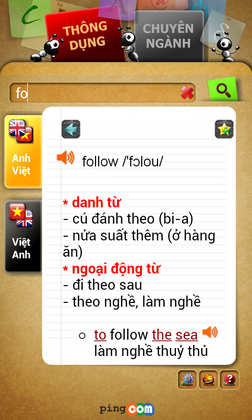
\includegraphics[width=0.30\textwidth] {hinh2_dist.png}
   \label{fig:Dict}}
\subfigure[Màn hình tài liệu]{
   
\includegraphics[width=0.30\textwidth] {hinh3_doc.png}
   \label{fig:Doc}}
\subfigure[Màn hình bài học]{
   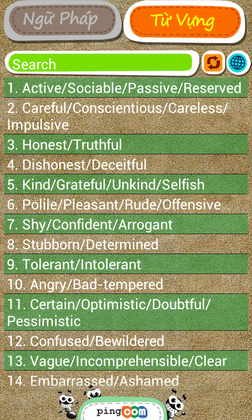
\includegraphics[width=0.30\textwidth] {hinh4_lesson.png}
   \label{fig:Lession}}
\subfigure[Màn hình luyện kĩ năng nghe và đọc]{
   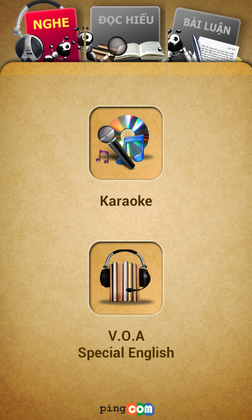
\includegraphics[width=0.30\textwidth] {hinh6_skills.png}
   \label{fig:Skill}}
\caption{Màn hình chính của chương trình }
\end{figure}

\subsection{Nhận xét chung}

Đa phần các phần mềm luyện nghe nói riêng và học tiếng Anh nói chung ở trên đều chỉ chạy ở một nền tảng nhất định, không có chức năng kết nối mạng để cập nhật nội dung bài học.

\section{Tổng kết chương}

Đa phần các chương trình luyện nghe tiếng Anh nói riêng và luyện học ngoại ngữ nói chung trên tablet thường chỉ chạy trên một nền tảng nhất định nào đó và thường là dạng ứng dụng offline. Còn đối với ứng dụng mà chúng em nghiên cứu và hiện thực sẽ có thể chạy trên nhiều nền tảng hệ điều hành khác nhau, và với sự hỗ trợ mạnh mẽ từ Moodle, sẽ giúp cho giáo viên soạn bài học được tốt hơn, tương tác với học viên tốt hơn, do ứng dụng chúng em cần phải có kết nối Internet để giảng viên có thể đổi nội dung bài học hay câu hỏi bất cứ lúc nào cũng được và ứng dụng trên tablet sẽ phải theo đó và hiện lên nội dung mới nhất mà giáo viên thay đổi, góp phần tạo nên sự tương tác giữa dạy và học, giữa giáo viên và học viên.

\chapter{Hệ Thống Luyện Nghe Tiếng Anh }

\ifpdf
    \graphicspath{{Chapter3/Chapter3Figs/PNG/}{Chapter3/Chapter3Figs/PDF/}{Chapter3/Chapter3Figs/}}
\else
    \graphicspath{{Chapter3/Chapter3Figs/EPS/}{Chapter3/Chapter3Figs/}}
\fi

\section{Đặt vấn đề}

Các tính năng cần thiết để xây dựng cho chương trình:

\quad - Luyện thi nghe IELTS (offline): một tính năng quan trọng của chương trình. Người sử dụng được làm bài thi nghe của bộ đề IELTS theo hai cách : luyện tập và thi thử.

\quad -	Luyện nghe online: đây là tính năng chủ chốt của chương trình. Người dùng sẽ đăng nhập vào hệ thống bằng tài khoản của Moodle, đăng nhập thành công thì người dùng có thể chọn khóa học mà mình muốn, chọn các bộ đề trong khóa học đó để luyện nghe.

\quad - Hệ thống Moodle sẽ làm nhiệm vụ quản lý tài khoản người dùng, quản lý nội dung bài học, lưu trữ các bộ đề. 

\quad -	Chức năng phụ: Xem thống kê kỹ năng: người sử dụng được xem lại điểm số những bài trắc nghiệm đã làm, với những đánh giá về kỹ năng nghe trong bài một cách khách quan nhất. Từ đó có thể rút ra những điểm yếu của bản thân trong việc luyện nghe.

\begin{figure}[!htb] 
\centering
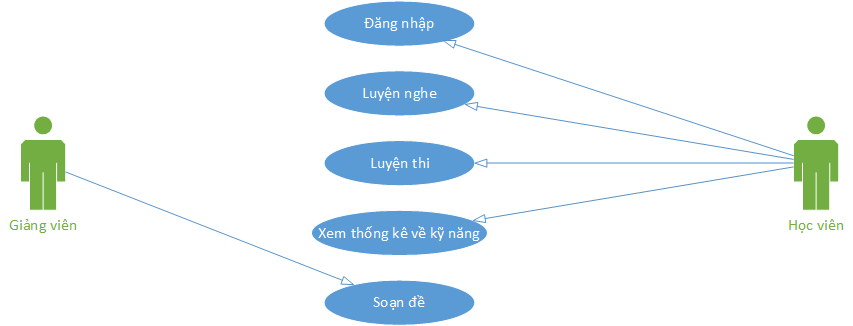
\includegraphics[width=0.8\textwidth]{usecase.png}
\caption{Sơ đồ usecase về các chức năng của ứng dụng}
\end{figure}

\section{Đề thi nghe IELTS}
\subsection{Tại sao lại chọn đề thi IELTS?}

IELTS là một bài kiểm tra về sự thành thạo Anh ngữ, được chấp nhận ở phần lớn các học viện ở Anh, Úc, Canada, Ireland, New Zealand, Nam Phi và ngày càng nhiều các học viện ở Mỹ cũng như nhiều tổ chức nghề nghiệp. Và IELTS đã trở thành hệ thống kiểm tra ngôn ngữ tiếng Anh dành cho bậc sau đại học và người di cư phổ biến nhất trên thế giới. Vì thế bài thi IELTS luôn có một độ khó nhất định và là tiêu chuẩn đánh giá khá chính xác và khách quan về kỹ năng tiếng Anh của người tham dự.

Các câu hỏi và phần audio của chương trình được trích từ các bộ đề thi IELTS phổ thông từ quyển Cambridge IELTS 9.\\
\\
\\
\\
\\
\\
\\
\\
\\
\\
\\
\\
\begin{figure}[!htb] 
\centering

\includegraphics[scale=0.8]{ielts9.png}
\caption{Bìa sách Cambridge IELTS 9 (Nguồn: covers.booktopia.com.au)}
\end{figure}

Vì nội dung chương trình chỉ mang tính chất tham khảo và không vì mục đích lợi nhuận nên nhóm đã sử dụng nội dung trong quyển sách nói trên. Nếu phát triển thành ứng dụng có tính phí, nhóm sẽ thay đổi với những nội dung có bản quyền.

\subsection{Cấu trúc bài thi}

Thời gian làm bài thi nghe là 40 phút với 40 câu hỏi, trong đó 30 phút là thời gian đoạn băng được phát cho bài thi nghe, và sẽ có 10 phút sau đó để thí sinh điền đáp án vào phiếu trả lời. Thí sinh sẽ nghe tất cả các câu hỏi và độ khó của từng câu sẽ tăng dần. Bài thi bao gồm nhiều dạng khác nhau như thông tin từ một người, cuộc đàm thoại của 2 hoặc nhiều người. Và thí sinh sẽ nghe nhiều giọng phát âm của nhiều quốc gia khác nhau. Thí sinh chỉ nghe được 1 lần. Tuy nhiên, bạn sẽ có thời gian để đọc câu hỏi và chuẩn bị câu trả lời. Bài thi nghe có 4 phần (số câu hỏi không được chia đều), nghe 1 lần và các đoạn nghỉ được ghi kèm trong băng hoặc đĩa. Cuối bài thi các thí sinh sẽ có 10 phút để ghi lại kết quả vào Phiếu trả lời câu hỏi.

\quad Phần 1: là các tình huống đời thường (đăng ký hoạt động, thuê nhà, nhập học) thường là 1 cuộc nói chuyện nhưng là hỏi đáp, và người đáp thường nói nhiều hơn.

\quad Phần 2: là các tình huống hướng dẫn và giới thiệu về 1 chủ đề quen thuộc (trường học, khu du lịch, chương trình ca nhạc, triển lãm,..) thường chỉ nói bởi 1 người.

\quad Phần 3: là các tình huống đối thoại giữa ít nhất là 2 người, đây là các cuộc thảo luận có tính chất học thuật hơn (Ví dụ: chọn chủ đề khóa luận, đề tài nghiên cứu khoa học).

\quad Phần 4: là 1 bài thuyết trình về 1 chủ đề học thuật, thường do 1 người nói và dùng nhiều từ ngữ mang tính chất học thuật.

\subsection{Cách tính điểm}

Bài thi Nghe bao gồm 40 câu. 1 câu trả lời đúng thí sinh sẽ được 1 điểm. Số điểm tối đa có thể đạt được là 40 cho từng bài thi. Thang điểm từ 1 – 9 sẽ được tính dựa trên số câu trả lời đúng. Cụ thể như sau:\\

\begin{figure}[htb] 
\centering
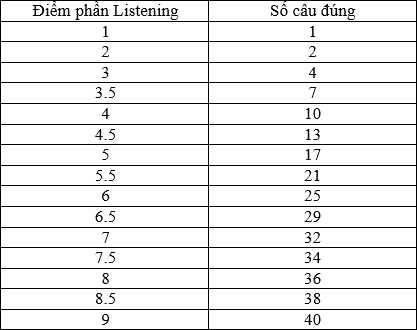
\includegraphics[scale=0.8]{score.png}
\caption{Thang điểm trong phần nghe của đề IELTS}
\end{figure}

\subsection{Các dạng câu hỏi}

Trong phần thi nghe của bài kiểm tra IELTS, thí sinh được nghe những đoạn audio về  3 đoạn hội thoại ở phần 1, 2, 3 và 1 chủ đề ở phần 4. Chủ yếu có các dạng câu hỏi sau:

\quad - Dạng câu hỏi điền từ vào chỗ trống: thí sinh sẽ điền những từ/cụm từ với số lượng chữ/chữ số được cho theo yêu cầu đề bài. Câu trả lời là chính xác nếu từ khóa của thí sinh trùng với từ khóa của đáp án. Trong một câu hỏi có thể có 2 ô trống để điền từ.

\begin{figure}[htb] 
\centering
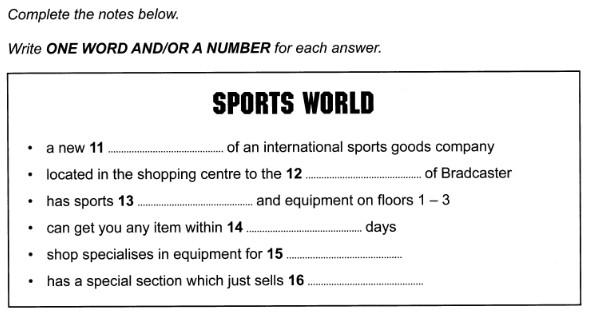
\includegraphics[scale=0.4]{ques_fill.png}
\caption{Mẫu câu hỏi điền từ vào mẩu thông tin}
\end{figure}

\quad - Ở dạng câu hỏi này, có thể có kiểu câu hỏi bắt thí sinh điền vào chỗ trống những phương án đề cho sẵn như TRUE, FALSE hoặc NOT GIVEN hoặc dạng điền thông tin vào sơ đồ, bảng biểu.

\begin{figure}[!htb] 
\centering
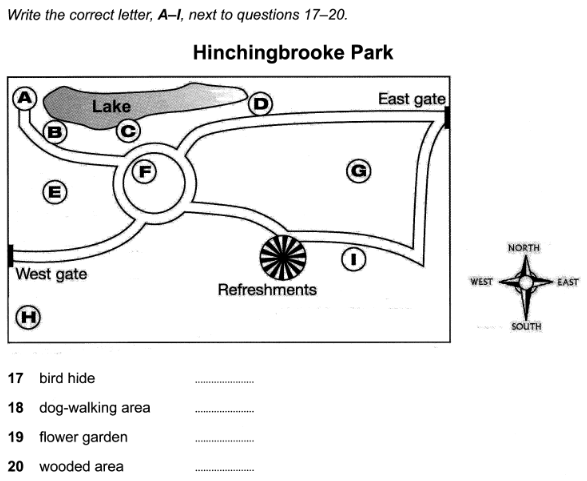
\includegraphics[scale=0.4]{ques_fill2.png}
\caption{Mẫu câu hỏi điền thông tin vào sơ đồ}
\end{figure}

\quad - Dạng câu hỏi trắc nghiệm: thí sinh sẽ nghe đoạn băng và trả lời câu hỏi với 3 phương án A, B, C với 1 lựa chọn thí sinh cho là đúng, hoặc 2 lựa chọn với dạng câu hỏi có 5 phương án A, B, C, D, E.

\begin{figure}[!htb] 
\centering
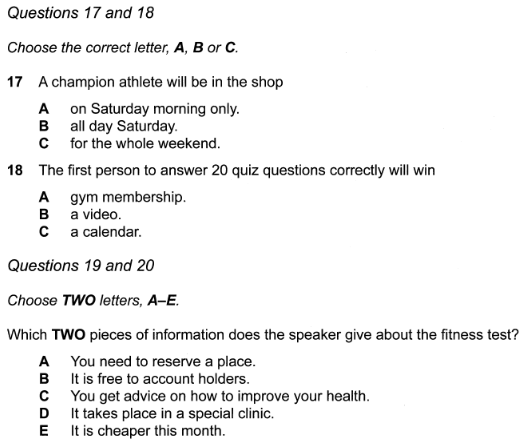
\includegraphics[scale=0.4]{ques_multi.png}
\caption{Mẫu câu hỏi trắc nghiệm}
\end{figure}

\subsection{Số hóa câu hỏi bằng các thành phần XML}

Dữ liệu của câu hỏi và các thông tin đi kèm, các phương án trả lời sẽ được lưu thành một file XML có cấu trúc đơn giản và được truyền về máy khách khi có yêu cầu. Sau đó, file XML sẽ được duyệt và hiển thị lên màn hình các thông tin được lưu trong file. Cấu trúc file XML như sau:

\begin{figure}[!htb] 
\centering
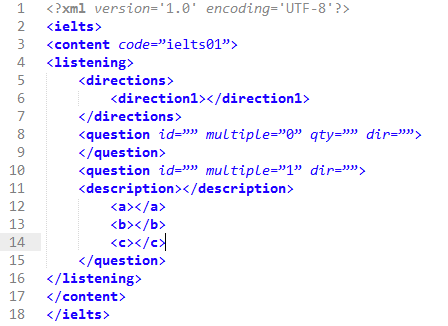
\includegraphics[scale=0.8]{xml.png}
\caption{Cấu trúc XML lưu trữ câu hỏi}
\end{figure}

Trong đó, chức năng của các thẻ như sau:

\quad - Thẻ <ielts> là thẻ root của file XML

\quad - Thẻ <content> có tham số code=”ielts01” chính là mã đề của đề hiện tại.

\quad - Thẻ <directions> chứa các chỉ dẫn làm bài của các câu hỏi, về loại câu hỏi và các thông tin cần thiết giúp thí sinh làm bài tốt hơn. Nhiều câu hỏi có thể có phần chỉ dẫn giống nhau.

\quad - Thẻ <question> chứa các thông tin về câu hỏi. Có 2 loại:

\quad \quad + Loại có tham số multiple=”0” là các dạng câu hỏi điền từ, với phần nội dung của thẻ là đoạn mã HTML đã được định dạng và được gói trong cú pháp CDATA. Những ô trống để thí sinh có thể điền từ vào được thể hiện trong mã HTML bằng thẻ <div id=”” class=” questext”></div>.

\quad \quad + Loại có tham số multiple=”1” là các dạng câu hỏi trắc nghiệm. Thẻ này có các thẻ con như <description> chứa thông tin câu hỏi và các thẻ <a>, <b>, <c> chứa các phương án lựa chọn trả lời. Đặc biệt là loại có tham số multiple=”2” là câu hỏi trắc nghiệm có 5 phương án lựa chọn với các thẻ phương án là <a>, <b>, <c>, <d> và <e>. Trong đó, thí sinh được chọn 2 phương án trả lời được cho là đúng.





\section{Thiết kế các tính năng ứng dụng}
Chương trình sẽ được phát triển theo mô hình truyền thông giữa Client và Server, trong đó, Moodle sẽ đóng vai trò làm Server, còn các tablet của người sử dụng là Client. Việc kết nối sẽ được thực hiện qua giao thức TCP/IP.
\newpage
\begin{figure}[!htb] 
\centering
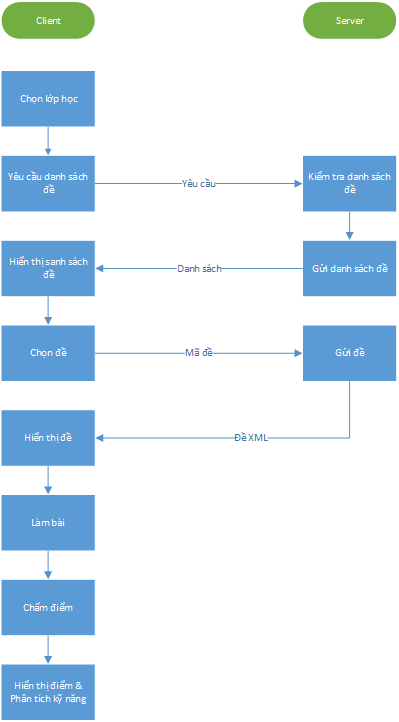
\includegraphics[width=0.6\textwidth]{flowchart.png}
\caption{Sơ đồ luồng chung của ứng dụng}
\end{figure}


\subsection{Thiết kế tính năng luyện nghe Offline}
Client sẽ kiểm tra danh sách đề thi trong dữ liệu chương trình. Sau đó sẽ hiển thị danh sách các đề hiện có.

Người sử dụng sẽ chọn đề. Nội dung đề được trả về là file XML và file audio.

Nội dung audio sẽ được phát, đồng thời client hiển thị nội dung câu hỏi cho người sử dụng làm bài.

\begin{figure}[!htb] 
\centering
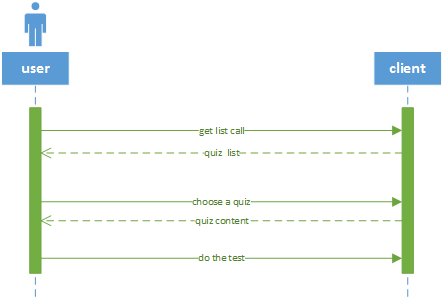
\includegraphics[width=0.8\textwidth]{getQuesSeq.png}
\caption{Sơ đồ sequence về hoạt động tải đề kiểm tra khi chạy offline}
\end{figure}

\subsection{Thiết kế tính năng đăng nhập và lấy token}

Khi bắt chương trình, giữa client và server sẽ thiết lập một kết nối truyền tải dữ liệu.

Sau khi người sử dụng nhập các thông tin tài khoản như tên tài khoản và mật khẩu, dữ liệu sẽ được gửi đến server.

Server sẽ kiểm tra thông tin và gửi trả về token xác thực phiên sử dụng của tài khoản nếu tên tài khoản và mật khẩu được gửi đến là đúng.

Kể từ đó, mỗi lời gọi đến server của client đều phải đính kèm token xác thực. Và server gửi trả thông tin được yêu cầu tương ứng.\\
\\
\\
\\
\begin{figure}[!htb] 
\centering
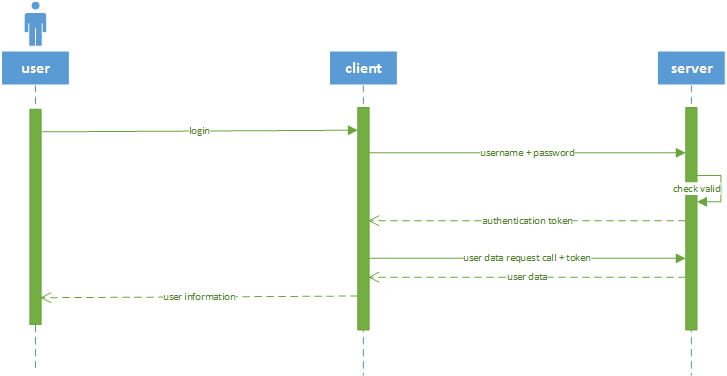
\includegraphics[width=0.8\textwidth]{loginSequence.png}
\caption{Sơ đồ sequence về hoạt động đăng nhập}
\end{figure}
\\

\subsection{Thiết kế tính năng lấy đề luyện nghe}

Sau khi đăng nhập thành công, client sẽ gửi yêu cầu danh sách đề thi kèm theo token cho server. Server sẽ gửi trả danh sách các đề đang có.

Người sử dụng sẽ chọn đề theo 3 mức độ khó. Id của đề sẽ được gửi lại cho server và server trả về nội dung đề là file XML và file audio.

Nội dung audio sẽ được phát, đồng thời client hiển thị nội dung câu hỏi cho người sử dụng làm bài.

\begin{figure}[!htb] 
\centering
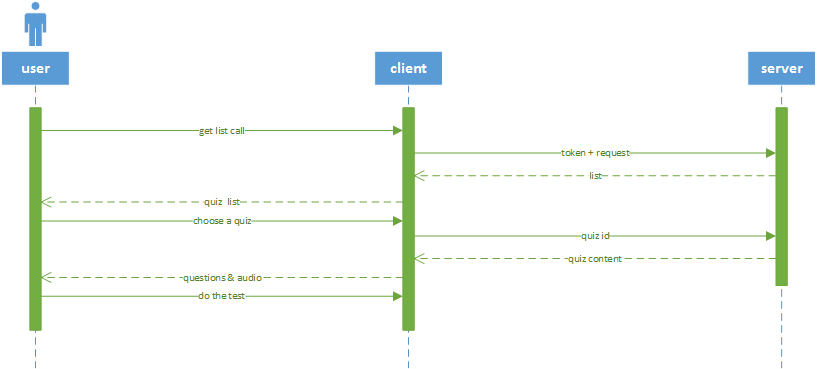
\includegraphics[width=0.8\textwidth]{getQuizSequence.png}
\caption{Sơ đồ sequence về hoạt động tải đề kiểm tra}
\end{figure}
\newpage

\subsection{Thiết kế tính năng chấm bài và đánh giá kỹ năng}

Sau khi người sử dụng làm bài xong và nhấn Submit, danh sách câu trả lời được gửi đến server.

Server sẽ dò và so sánh danh sách câu trả lời vừa nhận với danh sách đáp án đã lưu trước dựa theo mã đề. Câu trả lời đúng là câu trả lời có nội dung trùng với từ khóa trong đáp án.

Sau khi chấm, danh sách số câu trả lời đúng theo từng Section sẽ được gửi về cho client. Từ đó, client đánh giá được kỹ năng của người dùng dựa trên số điểm của mỗi Section với mỗi kỹ năng riêng.

\begin{figure}[!htb] 
\centering
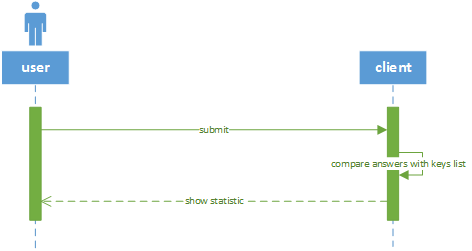
\includegraphics[width=0.8\textwidth]{getMarkSequenceOff.png}
\caption{Sơ đồ sequence về hoạt động nộp bài và chấm bài}
\end{figure}
\newpage

\section{Tổng kết chương}

Trong chương này, nhóm chúng em đã trình bày về đặc điểm của các câu hỏi trong bộ đề thi nghe IELTS để biểu diễn chúng dưới dạng dữ liệu và tìm ra cách thức tiếp cận, giải quyết các luồng hoạt động của chương trình.

Tuy nhiên, ở chương này, các bản thiết kế chỉ ở mức sơ bộ. Chúng em sẽ hoàn thiện các sơ đồ thiết kế này thành một ứng dụng hoàn chỉnh ở chương sau.


\chapter{Hiện Thực Hệ Thống Luyện Nghe Tiếng Anh}

\ifpdf
    \graphicspath{{Chapter4/Chapter4Figs/PNG/}{Chapter4/Chapter4Figs/PDF/}{Chapter4/Chapter4Figs/}}
\else
    \graphicspath{{Chapter4/Chapter4Figs/EPS/}{Chapter4/Chapter4Figs/}}
\fi

\section{Thiết kế lớp giao diện ứng dụng}

Các lớp giao diện được thiết kế tách rời nhằm đảm bảo tính thuận tiện và trực quan nhất cho ứng dụng.

\begin{figure}[!htb] 
\centering
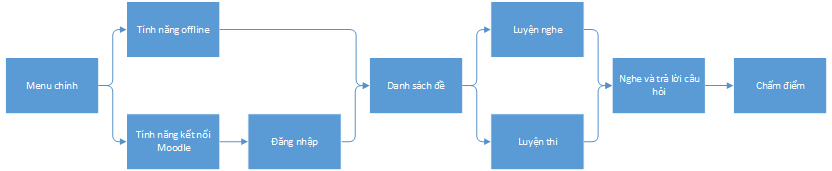
\includegraphics[width=0.9\textwidth]{gui.png}
\caption{Sơ đồ thiết kế giao diện chương trình}
\end{figure}

Sau khi lựa chọn tính năng chương trình, danh sách các đề sẽ được hiển thị cho người dùng chọn. 

Và sau khi đã chọn được một đề, cửa sổ chọn hình thức làm bài sẽ được xổ ra. 

Người dùng sẽ chọn hình thức luyện nghe hay luyện thi với tính năng bị hạn chế hơn. 

Giao diện làm bài hỗ trợ duyệt tới lui giữa các câu hỏi và duyệt nhanh giữa những câu còn chưa trả lời. 

Sau khi làm bài, phần chấm điểm sẽ hiển thị điểm số cùng các kỹ năng của người dùng. 

Sau đó là các kết quả làm bài ở những lần trước dưới dạng đồ thị để người dùng theo dõi quá trình ôn luyện của mình.

\section{Hiện thực tính năng luyện nghe offline}

Khi không có kết nối Internet, ứng dụng vẫn có thể hoạt động được nhờ việc sử dụng các dữ liệu mẫu đã được lưu trong chương trình dưới dạng XML. Người sử dụng vẫn có thể thực hiện các chức năng làm bài, chấm bài và xem kết quả một cách bình thường.

\begin{figure}[!htb] 
\centering
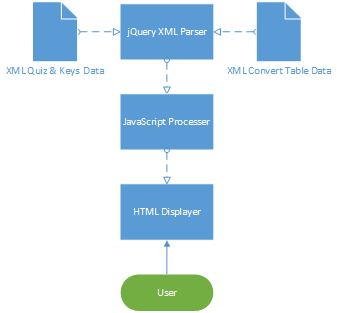
\includegraphics[width=0.5\textwidth]{offline.png}
\caption{Sơ đồ xử lý của các thành phần phía client tương ứng với chức năng nghe offline}
\end{figure}

Các bước hoạt động:

\quad - Mặc định, ứng dụng sẽ kiểm tra danh sách các đề có sẵn trong bộ nhớ. Sau khi người dùng chọn đề, nội dung các câu hỏi trong đề sẽ được hiển thị lần lượt lên màn hình, đồng thời nội dung audio cũng được chạy và bắt đầu tính thời gian làm bài.

\quad - Các câu trả lời của người dùng sẽ được lưu tạm vào SessionStorage, và sau khi có lệnh nộp bài, nội dung trong biến này sẽ được so sánh với các đáp án của đề tương ứng theo từng phần tử của mảng.

\quad - Chênh lệch nội dung của 2 mảng sẽ cho biết kết quả bài làm của người dùng. Kết quả này sẽ được lưu lại để làm thống kê về sau.


\section{Hiện thực tính năng kết nối với Moodle}
\subsection{Cấu trúc tương tác giữa client và server}

\begin{figure}[!htb] 
\centering
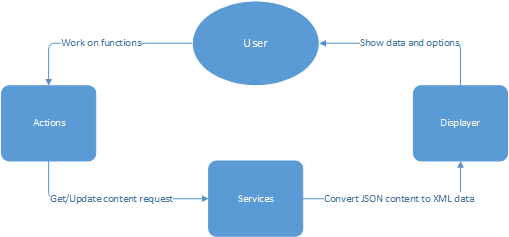
\includegraphics[width=0.8\textwidth]{server-client.png}
\caption{Sơ đồ cấu trúc ứng dụng ở cả server và client}
\end{figure}

Trong đó, chức năng cụ thể của từng khối như sau:

\quad - Actions: các thành phần JavaScript tập trung xử lý các tương tác của người dùng và chịu trách nhiệm trong việc gửi nhận dữ liệu.

\quad - Services: các dịch vụ của server Moodle giúp việc quản lý khóa học và đảm nhiệm việc cung cấp nội dung cho phía client.

\quad - Displayer: các thành phần HTML đảm nhiệm việc hiển thị thông tin về người dùng, khóa học và nội dung đề thi một cách trực quan và sinh động tới người dùng.

\subsection{Cấu hình trên moodle}

Trước hết ta phải ta phải đăng nhập vào Moodle với quyền admin.

Ta kích hoạt web service:

\quad - Vào Access Settings > Site administration > Advanced features
 
\quad - Chọn 'Enable web services' rồi chọn 'Save Changes'

Tạo web service:

\quad - Vào Access Settings > Site administration > Plugins > Web services > External services

\quad - Chọn Add new custom service

\quad - 'Authorised users only' - Nếu chọn, thì ta phải tự thêm vào các user được phép truy cập.
 
\quad - Gõ tên web service và chọn Enabled.

\quad - Click 'Add service'.

\begin{figure}[!htb] 
\centering
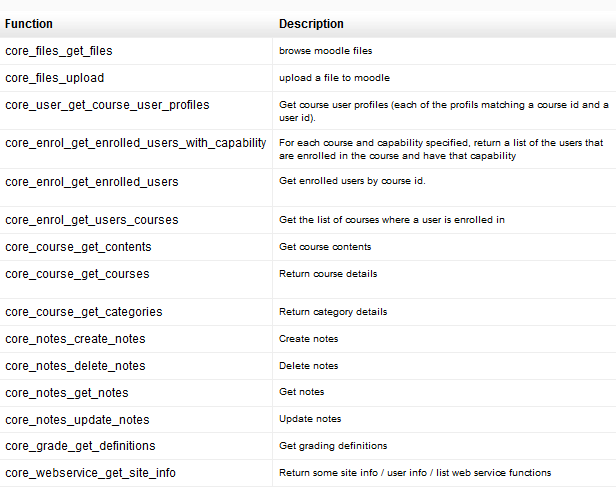
\includegraphics[width=0.8\textwidth]{wsfunction.png}
\caption{Một số web services cần dùng trong ứng dụng}
\end{figure}

Thêm các hàm cần sử dụng vào web service:

\quad - Chọn 'Add functions' link

\quad - Chọn các hàm cần sử dụng và click vào 'Add functions'

Để có thể gọi web sevice được ta cần phải truy cập vào cơ sở dữ liệu của Moodle, tìm đến table có tên là "mdl\_external\_services", thêm vào cột shortname tên web services.

\begin{figure}[!htb] 
\centering
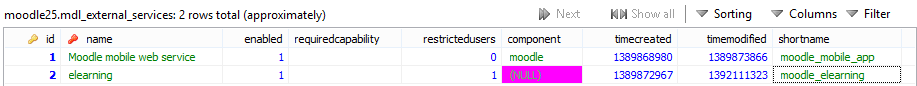
\includegraphics[width=0.8\textwidth]{addShortNameWS.png}
\caption{Cách thêm shortname cho web service}
\end{figure}
 
Bên cạnh sử dụng các hàm có sẵn của Moodle, ta cũng có thể tự tạo ra web service với các hàm do ta tự cài đặt nếu các hàm có sẵn không đáp ứng được nhu cầu.

\subsection{Mô hình xử lý trên client}

Client khi kết nối tới Moodle cũng có cơ chế làm việc tượng tự với khi đọc và xử lý dữ liệu offline. Nhưng nhờ kết nối tới máy chủ nên lượng dữ liệu sẽ phong phú và mang tính linh động cao hơn.

\begin{figure}[!htb] 
\centering
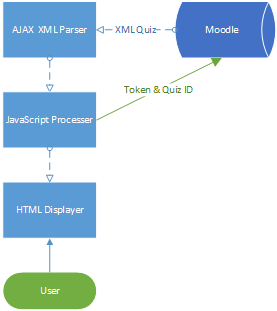
\includegraphics[width=0.5\textwidth]{client-onl.png}
\caption{Sơ đồ xử lý của các thành phần phía client tương ứng với chức năng luyện nghe có kết nối tới Moodle}
\end{figure}

Trong mục này, nhóm chúng em muốn giới thiệu về cách gọi các service của Moodle và cách xử lý dữ liệu trả về từ máy chủ trên client.

Để ứng dụng có thể tương tác với Moodle thì việc gửi và nhận dữ liệu đều liên quan đến một tham số là user token. Đó là một chuỗi ký tự đã được mã hóa, đặc trưng cho từng người sử dụng để xác thực phiên làm việc và quyền truy xuất đến service. Và để có được chuỗi token này, khi người sử dụng tiến hành đăng nhập ứng dụng phải gọi một HTTP request tới service cấp token với các tham số gồm username, password và tên của service.

Ta có ví dụ sau: \url{http://127.0.0.1/moodle25/login/token.php?username=09520266\&password=1qaz@WSX&service=moodle_elearning} sẽ đăng nhập với tên đăng nhập là “09520266” và mật khẩu là “1qaz@WSX”. Nếu đăng nhập thành công, server sẽ trả về chuỗi token ứng với phiên đăng nhập: 

“token: 247bc66c021e11f2e888f2476d71a44d” ứng với user "09520266".

Sau khi đã có chuỗi token, với mỗi lời gọi tới service cần phải đính chuỗi token đã lấy được như một tham số. Mỗi request sẽ có 2 phần chính:

\quad - Path: chứa đường dẫn của service

\quad - Query: chứa chuỗi token xác thực và các tham số cần thiết để lấy dữ liệu. Các tham số cách nhau bởi dấu “\&”.

Ví dụ: lời gọi \url{http://127.0.0.1/moodle25/webservice/rest/server.php?wsfunction=core_course_get_courses&wstoken=247bc66c021e11f2e888f2476d71a44d} sẽ gọi tới service “core\_course\_get\_courses” nhằm lấy về danh sách các khóa học của hệ thống. 

Trong đó, phần Path là \url{http://127.0.0.1/moodle25/webservice/rest/server.php} và phần Query có 2 tham số là “wsfunction=core\_course\_get\_courses” và “wstoken=247bc66c021e11f2e888f2476d71a44d”.

Như vậy, khi ghép tham số “wsfunction” với tên các service đã liệt kê bên trên, ta được một lời yêu cầu tới máy chủ Moodle để gọi service tương ứng và nhận dữ liệu XML với các thành phần key-value mà máy chủ trả về.


\section{Hiện thực việc triển khai ứng dụng}
Một số hình ảnh thực tế của ứng dụng mà nhóm khóa luận đã thực hiện được:

\begin{figure}[!htb] 
\centering
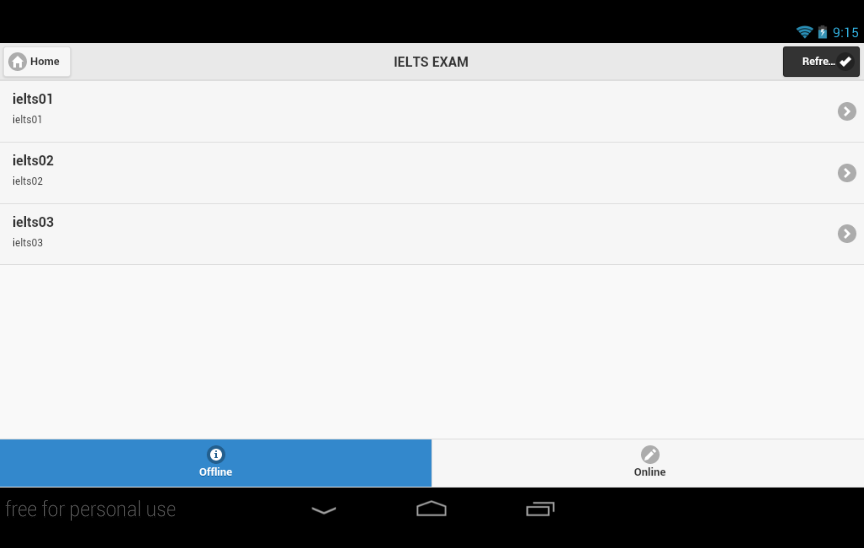
\includegraphics[width=0.8\textwidth]{1list_screen.png}
\caption{Màn hình danh sách các bài luyện nghe offline}
\end{figure}

\newpage

\begin{figure}[!htb] 
\centering
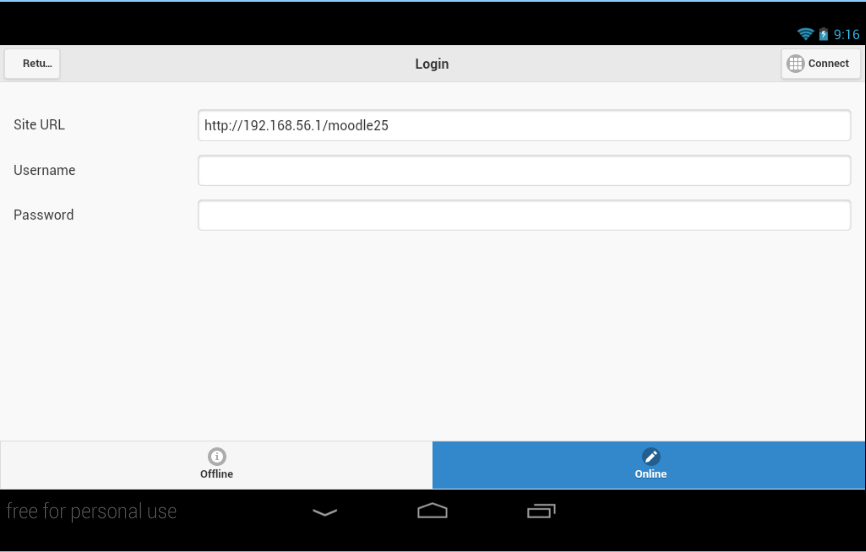
\includegraphics[width=0.8\textwidth]{2login_screen.png}
\caption{Màn hình đăng nhập vào Moodle}
\end{figure}

\begin{figure}[!htb] 
\centering
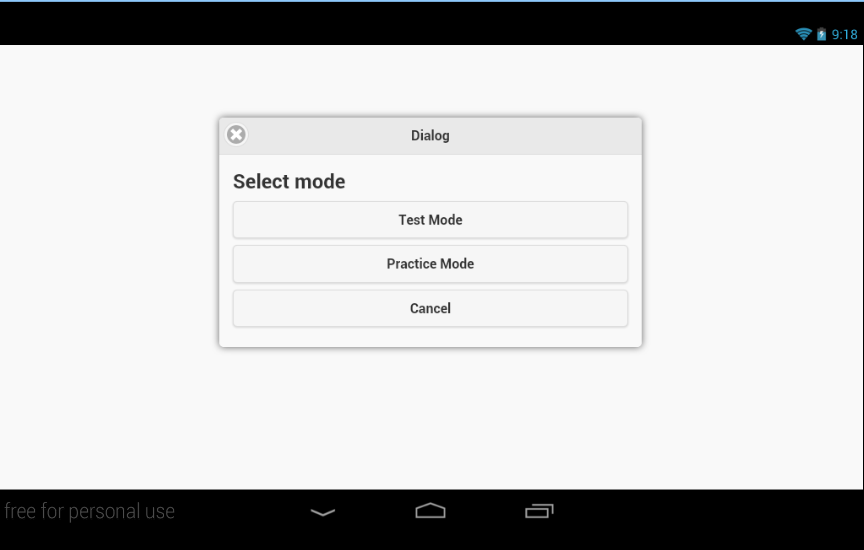
\includegraphics[width=0.8\textwidth]{3select_mode.png}
\caption{Màn hình chọn chế độ}
\end{figure}

\newpage

\begin{figure}[!htb] 
\centering
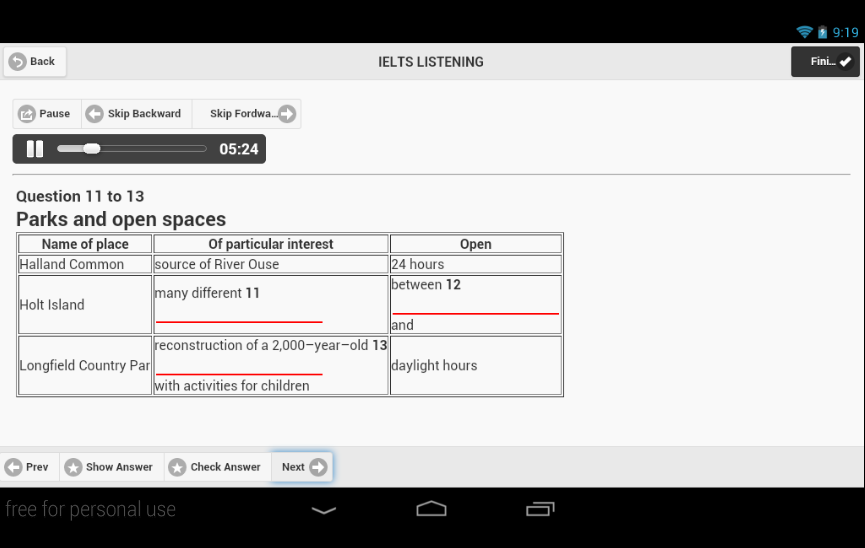
\includegraphics[width=0.8\textwidth]{4pracmode_1.png}
\caption{Màn hình làm bài với dạng câu hỏi điền từ}
\end{figure}

\begin{figure}[!htb] 
\centering
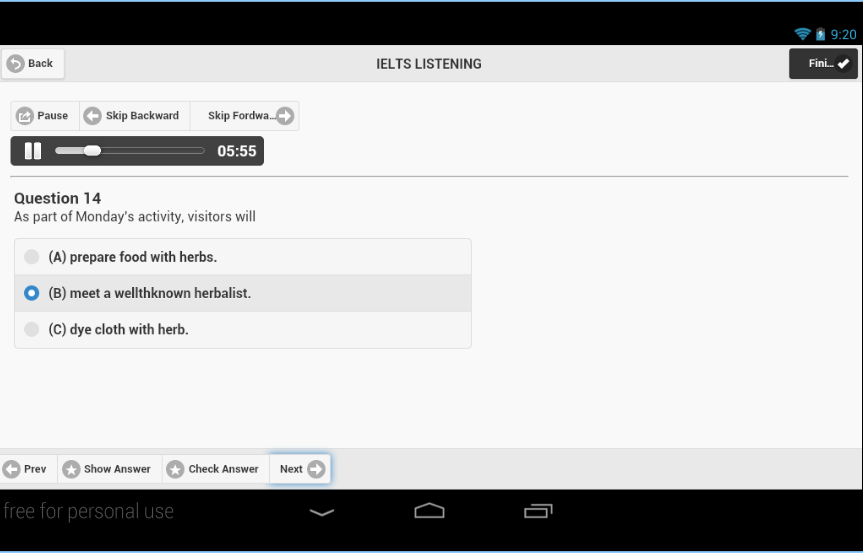
\includegraphics[width=0.8\textwidth]{5pracmode_2.png}
\caption{Màn hình làm bài với dạng câu hỏi trắc nghiệm}
\end{figure}

\newpage

\begin{figure}[!htb] 
\centering
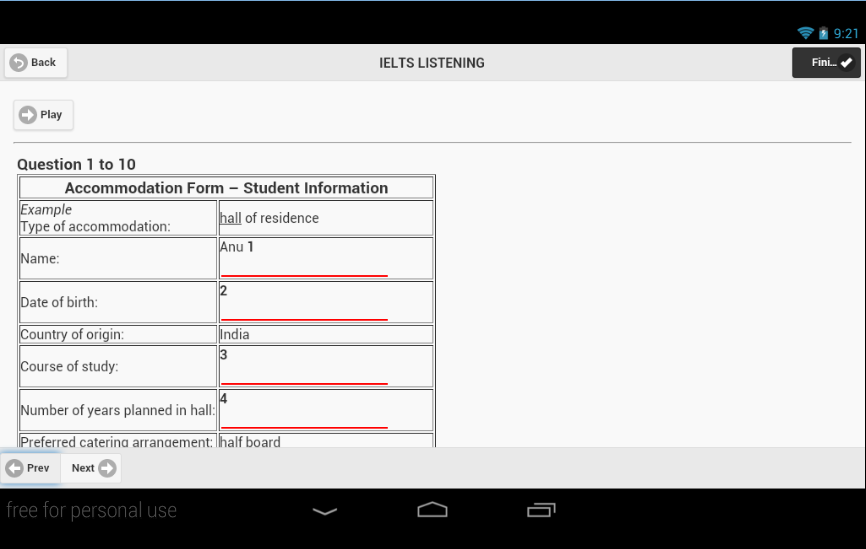
\includegraphics[width=0.8\textwidth]{6testmode.png}
\caption{Màn hình chức năng luyện nghe ở chế độ thi thử}
\end{figure}

\begin{figure}[!htb] 
\centering
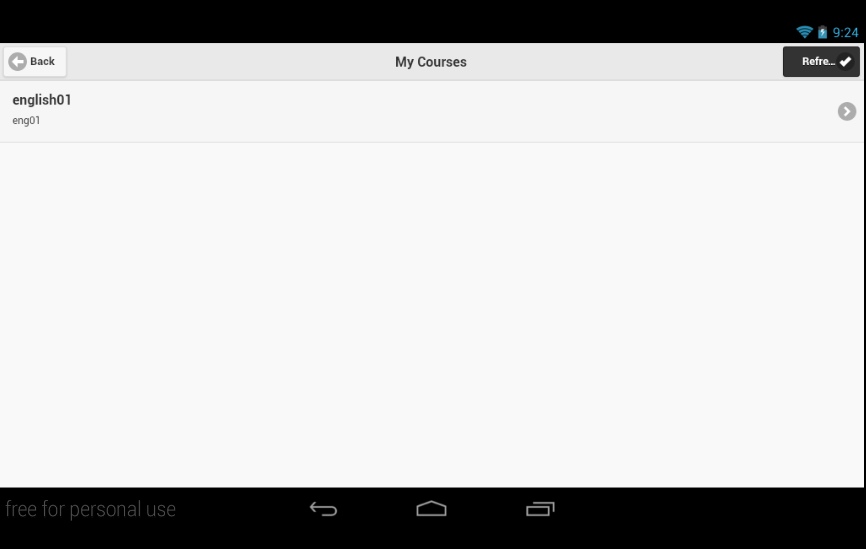
\includegraphics[width=0.8\textwidth]{7listcourse.png}
\caption{Màn hình danh sách khóa học có trên Moodle}
\end{figure}

\newpage

\begin{figure}[!htb] 
\centering
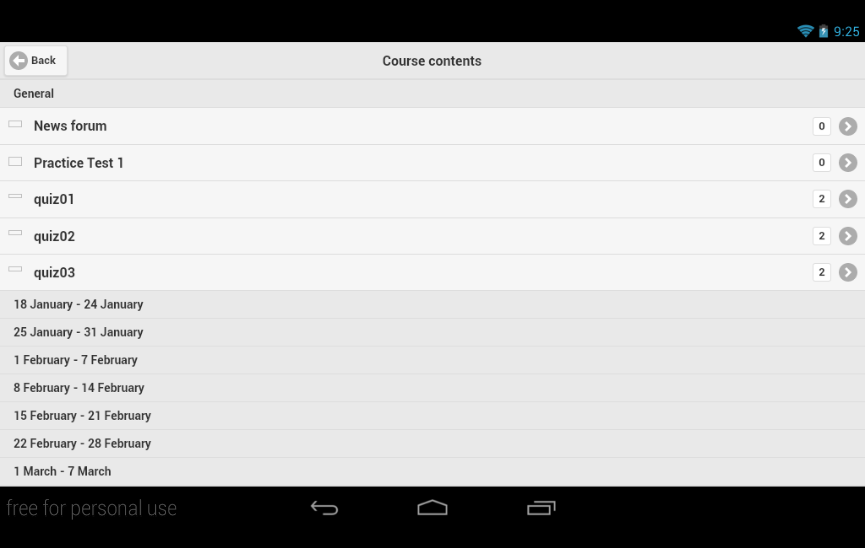
\includegraphics[width=0.8\textwidth]{8coursecontent.png}
\caption{Màn hình nội dung khóa học - liệt kê các bài nghe do giáo viên soạn}
\end{figure}

\begin{figure}[!htb] 
\centering
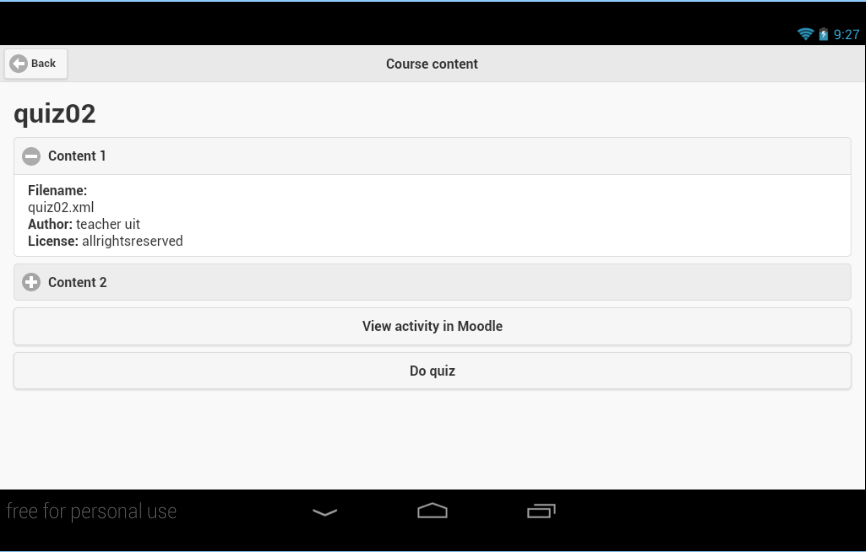
\includegraphics[width=0.8\textwidth]{9quizcontent.png}
\caption{Màn hình nội dung một bài luyện nghe - Nhấn nút "Do quiz" để luyện tập}
\end{figure}

\newpage

\section{Tổng kết chương}

Trải qua bốn chương mà chúng em trình bày, khóa luận đã nghiên cứu và xây dựng được chương trình luyện nghe tiếng Anh theo cấu trúc đề thi IELTS trên máy tính bảng, hỗ trợ hai chức năng chính đó là luyện nghe offline không cần đến Internet, luyện nghe online thông qua kết nối đến Moodle.

Điểm nổi bật của ứng dụng mà chúng em xây dựng so với các ứng dụng tương tự khác, đó là:

\quad - Khả năng chạy được trên nhiều nền tảng di động khác nhau như iPhone, iPad, Android, Windows Phone,...

\quad - Tính năng kết nối đến Moodle tạo nên sự phong phú về nội dung bài học.

Bên cạnh đạt được những kết quả tốt đẹp, khóa luận cũng còn mắc phải một số hạn chế. Chúng em xin được phép trình bày rõ về những hạn chế, khó khăn trong chương cuối cùng - kết luận và hướng phát triển.

\def\baselinestretch{1}
\chapter{Kết Luận và Hướng Phát Triển}
\ifpdf
    \graphicspath{{Conclusions/ConclusionsFigs/PNG/}{Conclusions/ConclusionsFigs/PDF/}{Conclusions/ConclusionsFigs/}}
\else
    \graphicspath{{Conclusions/ConclusionsFigs/EPS/}{Conclusions/ConclusionsFigs/}}
\fi

\def\baselinestretch{1.66}
 

\section{Kết luận}

Đến đây, chúng em xin đi đến kết luận. Về cơ bản hệ thống của chúng em hầu như hoàn thiện ở phía Client và giúp người sử dụng có khả năng chọn và nghe bài học, trả lời câu hỏi và xem điểm. Còn về phía Server, chúng em chưa hiện thực được ý tưởng một cách đầy đủ, chỉ mới xây dựng được chức năng chọn và tải đề soạn theo cấu trúc XML dựa vào sự hỗ trợ của Web service trên Moodle chứ chưa thật sự tạo ra riêng một hệ thống Web services phục vụ nhu cầu.

Tuy ứng dụng chưa thật sự hoàn chỉnh về mặt chương trình, nhưng nhóm khóa luận tin rằng nếu ứng dụng luyện nghe tiếng Anh này khi hoàn thiện thì khả năng được áp dụng vào thực tiễn rất cao. Chúng em tin rằng ứng dụng sẽ giúp người học nâng cao được kỹ năng nghe hiểu tiếng Anh tốt hơn và thuận tiện hơn.
 
\section{Hạn chế, khó khăn}

Do HTML5 chưa phải là một chuẩn chung của nên nhiều thiết bị còn chưa tương thích và chưa hỗ trợ đầy đủ, nên sẽ có thiết bị sẽ không thể chạy được ứng dụng Client. Qua khảo sát thực tế, chương trình chúng em chạy ổn định trên các thiết bị iPad của Apple và tablet Android.

Trong quá trình phát triển ứng dụng dùng nền tảng IBM Worklight v6, nhóm khóa luận còn gặp trục trặc về nhiều lỗi phát sinh.

\section{Phương hướng phát triển}

Chúng em đề ra phương hướng để phát triển hệ thống học tập như sau:

\quad - Thiết kế lại giao diện để thân thiện hơn với người dùng.

\quad - Thêm chức năng xem từ mới của bài nghe và ghi chú cho người học.

\quad - Cài đặt Web services có khả năng chuyển đổi các câu hỏi trong Quiz Activities trên Moolde thành file XML/JSON, giúp cho việc soạn đề của giáo viên trở nên nhẹ nhàng hơn thay vì phải soạn đề trực tiếp thành file XML.

Trong tương lai xa hơn nữa, hệ thống của chúng em hy vọng sẽ phát triển thành một thư viện e-learning trên máy tính bảng, để có thể tùy chỉnh giảng dạy các môn học khác nhau chứ không chỉ là luyện nghe tiếng Anh với nguồn dữ liệu đồ sộ và xây dựng được một cộng đồng đông đảo, giúp cho việc hoàn thiện chương trình và góp phần nâng cao hơn nữa nền giáo dục nước nhà.

 
%%% ----------------------------------------------------------------------

% ------------------------------------------------------------------------

%%% Local Variables: 
%%% mode: latex
%%% TeX-master: "../thesis"
%%% End: 


\backmatter  
\appendix
%\chapter{Phụ lục A}

Đây là phụ lục A 

% ------------------------------------------------------------------------

%%% Local Variables: 
%%% mode: latex
%%% TeX-master: "../thesis"
%%% End: 

%\chapter{Phụ lục B}
Đây là phụ lục B 
% ------------------------------------------------------------------------

%%% Local Variables: 
%%% mode: latex
%%% TeX-master: "../thesis"
%%% End: 

\chapter{Tài Liệu Tham Khảo}

\textbf{Sách tham khảo:}\\

[1] Cambridge ESOL (2013),\textit{Cambridge IELTS 9 Student's Book with Answers}, Cambridge University Press.

[2] Christopher Schmitt \& Kyle Simpson (2011), \textit{HTML5 Cookbook}, O'Reilly Media.

[3] IBM Corporation (2013), \textit{IBM Worklight Version 6.1.0 Information Center}, IBM Corporation. 

[4] Jonathan Stark (2010), \textit{Building Android Apps with HTML, CSS, and JavaScript , First Edition}, O'Reilly. Media.\\



\textbf{Website:}\\

[5] Grace Walker, Các quy tắc cơ bản của HTML5, đường dẫn \url{http://www.ibm.com/developerworks/vn/library/wa-html5fundamentals/}, tham khảo ngày 15/11/2013.

[6] Moodle, \textit{Web services FAQ}, đường dẫn \url{http://docs.moodle.org/25/en/Web_services_FAQ}, tham khảo ngày 15/11/2013.

[7] Moodle, \textit{Enable mobile web services}, đường dẫn \url{http://docs.moodle.org/25/en/Enable_mobile_web_services}, tham khảo ngày 15/11/2013.

[8] Moodle, \textit{Using web services}, đường dẫn \url{http://docs.moodle.org/25/en/Using_web_services}, tham khảo ngày 15/11/2013.

[9] Moodle, \textit{Creating a web service client}, đường dẫn \url{http://docs.moodle.org/dev/Creating_a_web_service_client} , tham khảo ngày 15/11/2013.

[10] The jQuery Foundation, jQuery API, đường dẫn \url{http://api.jquery.com/} , tham khảo ngày 15/11/2013.
  
[11] The jQuery Foundation, jQuery Mobile Demos, đường dẫn  \url{http://demos.jquerymobile.com/1.4.0/}, tham khảo ngày 15/11/2013.

[12] The Refsnes Data, AJAX Introduction, đường dẫn \url{http://www.w3schools.com/ajax/ajax_intro.asp}, tham khảo ngày 15/11/2013.

[13] W3C, \textit{Web Storage} , đường dẫn \url{http://www.w3.org/TR/webstorage/}, tham khảo ngày 15/11/2013.

[14] W3C, \textit{HTML/Elements/audio} , đường dẫn\url{http://www.w3.org/wiki/HTML/Elements/audio}, tham khảo ngày 15/11/2013.

[15] Wikipedia, \textit{HTML5}, đường dẫn \url{http://en.wikipedia.org/wiki/HTML5}, tham khảo ngày 15/11/2013.

[16] Wikipedia, \textit{JavaScript}, đường dẫn \url{http://en.wikipedia.org/wiki/JavaScript}, tham khảo ngày 15/11/2013. \\

\textbf{Source code tham khảo:}\\

[17] Juan Leyva (2012), Unofficial Moodle Mobile app, đường dẫn \url{https://github.com/jleyva/umm} , tham khảo ngày 10/12/2013.


%1\bibliographystyle{Classes/jmb} % bibliography style
%\renewcommand{\bibname}{Tài Liệu Tham Khảo} % changes default name Bibliography to References
\bibliography{security} % References file

\end{document}